%Pakete;
%A4, Report, 12pt
\documentclass[ngerman,a4paper,12pt]{scrreprt}
\usepackage[a4paper, right=20mm, left=20mm,top=30mm, bottom=30mm, marginparsep=5mm, marginparwidth=5mm, headheight=7mm, headsep=15mm,footskip=15mm]{geometry}

%Papierausrichtungen
\usepackage{pdflscape}
\usepackage{lscape}

%pdf include
\usepackage{pdfpages}

%Deutsche Umlaute, Schriftart, Deutsche Bezeichnungen
\usepackage[utf8]{inputenc}
\usepackage[T1]{fontenc}
\usepackage[ngerman]{babel}

%quellcode
\usepackage{listings}

%tabellen
\usepackage{tabularx}

%listen und aufzählungen
\usepackage{paralist}

%farben
\usepackage[svgnames,table,hyperref]{xcolor}

%font
\usepackage{helvet}
\renewcommand{\familydefault}{\sfdefault}

%Abkürzungsverzeichnisse
\usepackage[printonlyused]{acronym}

%Bilder
\usepackage{graphicx} %Bilder
\usepackage{float}	  %"Floating" Objects, Bilder, Tabellen...

%Kopf- /Fusszeile
\usepackage{fancyhdr}
\usepackage{lastpage}

\pagestyle{fancy}
\fancyhf{} %alle Kopf- und Fußzeilenfelder bereinigen
\fancyhead[L]{Semesterarbeit} %Kopfzeile links
\fancyhead[C]{\project} %Kopfzeile mitte
\fancyhead[R]{Seite \thepage/\pageref{LastPage}} %Kopfzeile rechts
\renewcommand{\headrulewidth}{0.4pt} %obere Trennlinie
\fancyfoot[L]{\jobname} %Fusszeile links
\fancyfoot[C]{Version: \versionnumber} %Fusszeile mitte
\fancyfoot[R]{\today{}} %Fusszeile rechts
\renewcommand{\footrulewidth}{0.4pt} %untere Trennlinie

%Kopf-/ Fusszeile auf chapter page
\fancypagestyle{plain} {
	\fancyhf{} %alle Kopf- und Fußzeilenfelder bereinigen
	\fancyhead[L]{Semesterarbeit} %Kopfzeile links
	\fancyhead[C]{\project} %Kopfzeile mitte
	\fancyhead[R]{Seite \thepage/\pageref{LastPage}} %Kopfzeile rechts
	\renewcommand{\headrulewidth}{0.4pt} %obere Trennlinie
	\fancyfoot[L]{\jobname} %Fusszeile links
	\fancyfoot[C]{Version: \versionnumber} %Fusszeile mitte
	\fancyfoot[R]{\today{}} %Fusszeile rechts
	\renewcommand{\footrulewidth}{0.4pt} %untere Trennlinie
}

\usepackage{changepage}

%links, verlinktes Inhaltsverzeichnis, PDF Inhaltsverzeichnis
\usepackage[bookmarks=true,
bookmarksopen=true,
bookmarksnumbered=true,
breaklinks=true,
colorlinks=true,
linkcolor=black,
anchorcolor=black,
citecolor=black,
filecolor=black,
menucolor=black,
pagecolor=black,
urlcolor=black
]{hyperref} % Paket muss unbedingt als letzes eingebunden werden!

%Dokumenteigenschaften
\providecommand{\project}{WebRTC VoIP Applikation}
\author{Tobias Blaser, Jannis Grimm}
\providecommand{\room}{1.258}
\providecommand{\teacher}{Luc Bläser}
\title{\documentType \project}
\date{\today{}, Rapperswil}

\usepackage{csvsimple}

%Dokumenteigenschaften
\providecommand{\documentType}{Projektdokumentation}
\providecommand{\versionnumber}{1.9}

\begin{document}

%Titel und Inhaltsverzeichnis
\thispagestyle{empty}
\begin{titlepage}
\begin{figure}[htp]
		
\includegraphics[height=2.5cm]{../projektdokumentation/img/hsrLogo.jpg}
	\end{figure}	
	
	\begin{center}

		\vspace*{1cm}
		{\fontsize{32}{40} \selectfont \textbf{\project} \\[10mm]}
	
		\begin{figure}[htp]
			\centering
			
\includegraphics[scale=0.60]{../img/icon-js-voip.png}
		\end{figure}		
		\vspace*{20mm}	
	
		{\fontsize{32}{40} \selectfont \textbf{Studienarbeit} \\[10mm]}
	
		{\fontsize{18}{20} \selectfont 
			Abteilung Informatik\\
			Hochschule für Technik Rapperswil \\
				
			\vspace*{1cm}
			Herbstsemester 2013\\
		}
		
		\vspace*{2cm}
		Tobias Blaser, Jannis Grimm\\
		Betreuer: Prof. Dr. Luc Bläser

	\end{center}
\end{titlepage}
\clearpage


\includepdf[pages=-]{../projektdokumentation/media/Aufgabenstellung.pdf}
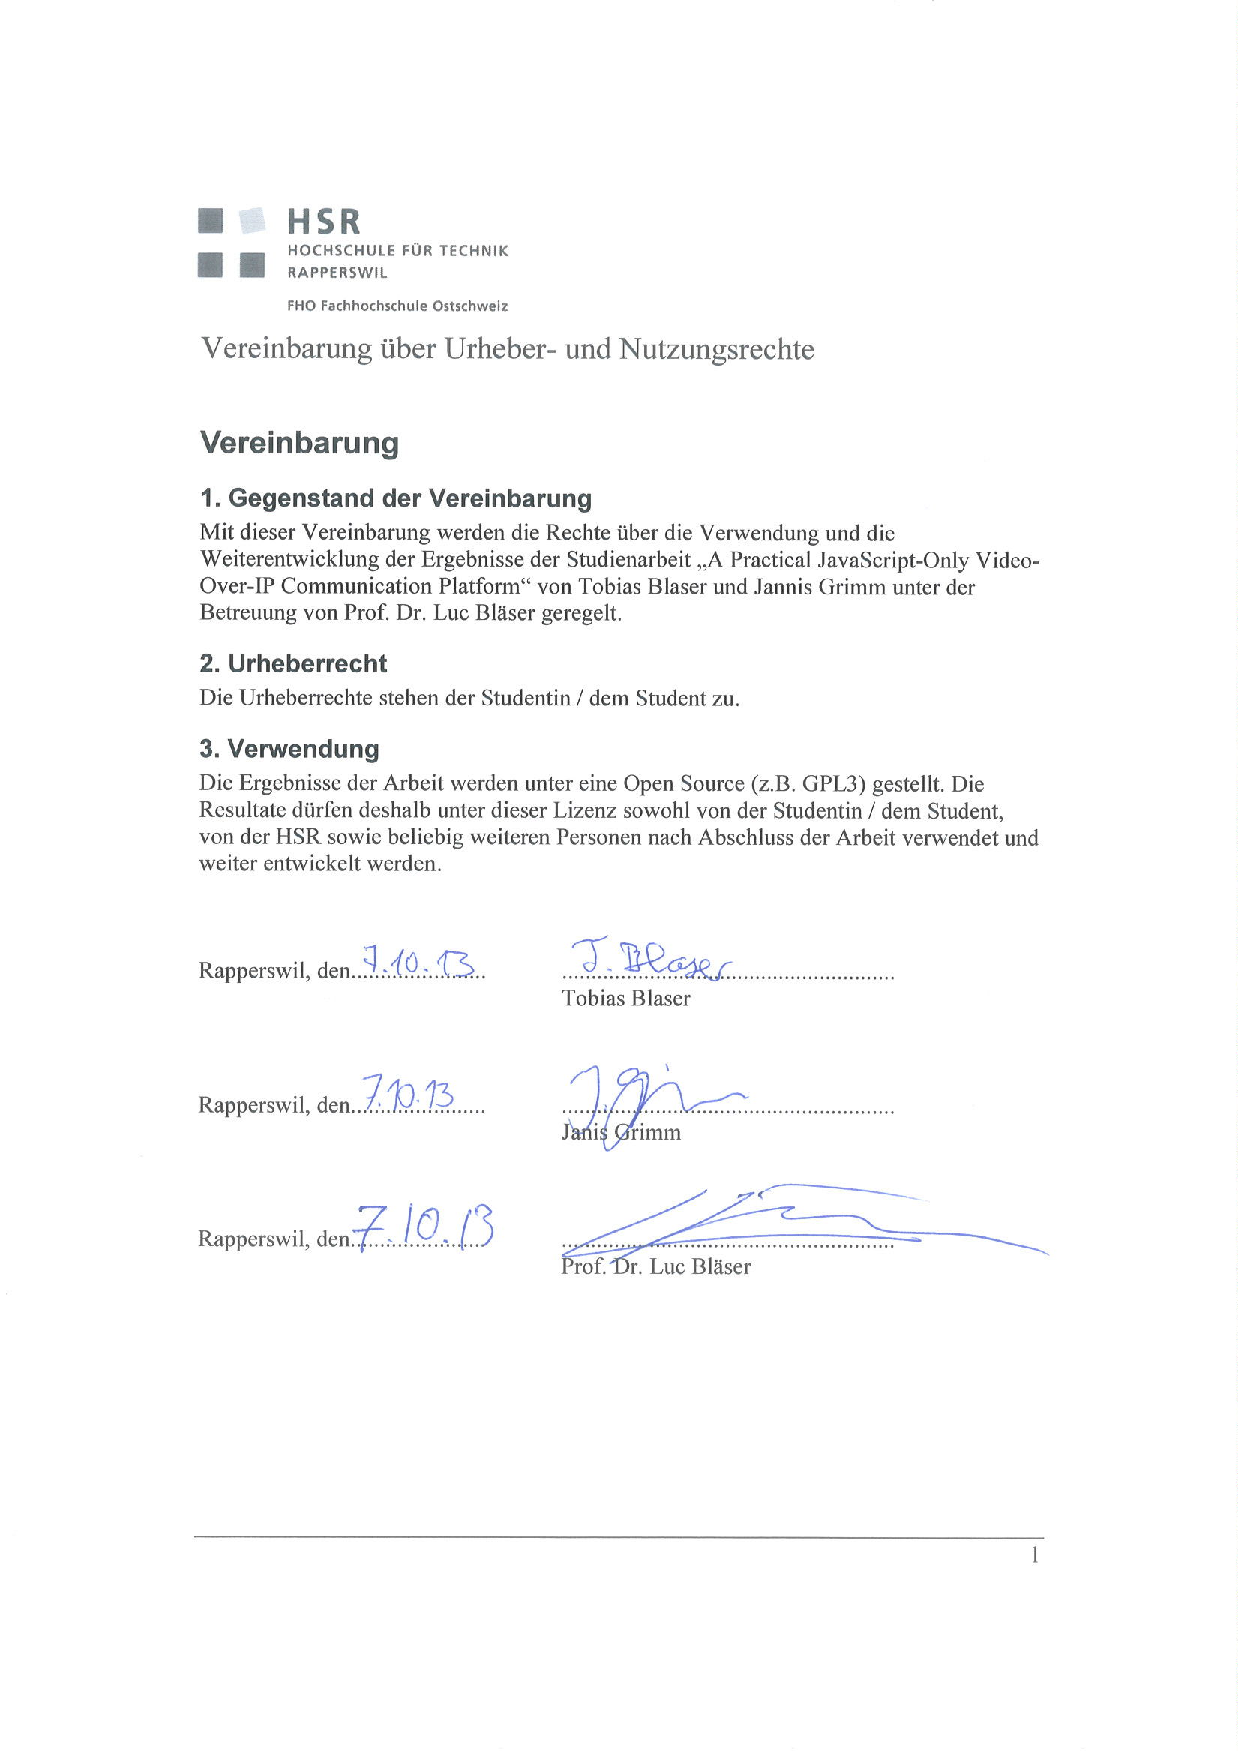
\includepdf[pages=-]{../projektdokumentation/media/Nutzungsvereinbarung.pdf}

\includepdf[pages=-]{../projektdokumentation/media/Eigenstaendigkeitserklaerung.pdf}


\chapter*{Änderungsnachweis}
\begin{tabularx}{\textwidth}{|cXlr|} % Versionstabelle, Rahmen links und rechts
		\hline
		\textbf{Version} & \textbf{Änderung} & \textbf{Autor} & \textbf{Datum}\\
		\hline
		1.0 & Dokumentenentwurf & Tobias Blaser & 04.11.13\\
		1.1 & Hinzufügen zusätzlicher Dokumente & Tobias Blaser & 07.11.13\\
		1.2 & Verfassen von Vision und Qualitätsmanagement & Tobias Blaser \& Jannis Grimm & 19.11.13\\
		1.3 & Lektorat & Jannis Grimm & 22.11.13\\
		1.4 & Tobias Blaser & Überarbeitung verschiedener Kapitel & 22.11.13\\
		1.5 & Doku Review & Jannis Grimm & 22.11.13\\
		1.6 & Abstract \& Management Summary & Tobias Blaser, Jannis Grimm & 10.12.13\\
		1.7 & Performanceanalyse & Tobias Blaser, Jannis Grimm & 12.12.13\\
		1.8 & Firewall Testing, Erkenntnisse, Überarbeitungen & Jannis
		Grimm & 14.12.13\\
		\versionnumber & Schnittstellen und Protokolle & Tobias Blaser & 15.12.13\\
		\hline
\end{tabularx}

% Inhaltsverzeichnis
\tableofcontents

% abstract, management summary, vision
\chapter{Abstract}

Ziel der Studienarbeit "`A Practical JavaScript-Only Video-Over-IP
Communication Plattform"' war die Entwicklung einer JavaScript-Applikation zur Audio- und Videokommunikation, die ausschliesslich im Browser läuft. Benutzer müssen keine Software auf ihrem Endgerät installieren, um die Applikation nutzen zu können.
Teil der Arbeit waren die Untersuchungen des aktuellen Standes der Technologien
und der notwenigen Schnittstellen, die Umsetzung von Referenzimplementationen
der eigenen Schnittstellen, sowie eine Analyse der Performance.

Die Benutzeroberfläche wurde sowohl für Desktop wie Mobilgeräte konzipiert und übersichtlich gestaltet. Unterstützt werden Benutzerkonten sowie Import von Kontaktdaten.
Über Schnittstellen kann die Applikation um eigene Kontaktdatenformate und Verbindungsmechanismen erweitert werden.

Die Unterstützung durch die Browser ist noch sehr unterschiedlich. Nur neuere Chrome-, Firefox- und Opera-Versionen unterstützen die Schnittstellen, wobei die Unterstützung experimentell ist und entsprechend variiert. Mediacodierung und Verschlüsselung verbrauchen auch noch spürbar viel Rechenleistung. Die automatische Datenratenskalierung wird bereits durch alle getesteten Browser unterstützt.

Die Technologien hinter den JavaScript-Schnittstellen setzen Protokolle wie STUN
oder ICE ein, die von stark restriktiven Firewalls blockiert werden. In
Netzwerkumgebungen wie Heimnetzwerken oder kleineren, schwach reglementierten Firmennetzwerken, sowie im Mobilfunknetz stellt dies jedoch keine Probleme dar.

Wir haben es erfolgreich geschafft, eine JavaScript-basierte
Videokommunikationsplattform mit dem aktuellen Stand der Browsertechnologie aufzubauen. Alle browserseitig notwendigen Schnittstellen existieren und funktionieren bereits. Trotzdem ist deren Umsetzung noch experimentell, was sich vor allem durch den Ressourcenverbrauch bemerkbar macht.

Mit der erreichten Lösung sind wir sehr zufrieden. Wir haben die gesteckten
Ziele sogar übertroffen, indem wir die Videokommunikation um einen Chat erweitert haben.

\chapter{Management Summary}

\section{Ausgangslage}
Videokommunikation wird bereits seit Jahrzehnten gehypt, verbreitet sich jedoch erst seit einigen Jahren. 
Besonders bekannt sind hier die Produkt Skype von Skype Technologies, Google Hangout sowie Facetime von Apple.
Diese mittlerweile sehr verbreitete Produkte benötigen alle die Installation einer Softare auf jedem Endgerät. Die Produkte verwenden eigene Protokolle, sodass untereinander nicht kommuniziert werden kann. Bietet der Anbieter keine Applikation für eine bestimmte Plattform, kann diese nicht zur Kommunikation genutzt werden.

Daneben gibt es SIP als offnenen Standard, der sich in vielen Firmen etabliert hat und für IP-Telefonie genutzt wird. Auch für SIP wird auf jedem Endgerät eine entsprechende Software benötigt, Telefonie zwischen verschiedenen SIP-Providern ist möglich.

Videokommunikation ohne Installation einer Software war bisher nicht möglich. Neue Browser unterstützen nun jedoch entsprechende Technologien.


\section{Vorgehen}
In der Anfangsphase des Projektes lag der Schwerpunkt darauf, die Grenzen der Technologie abzustecken, da die Schnittstellen sich noch in Entwicklung befinden und von den Browsern erst seit einiger Zeit unterstützt werden.

In der anschliessenden Phase ging es darum, mit den Prototypen der ersten Phase eine rudimentäre Applikation umzusetzen, die bereits Videokommunikation und Import von Kontaktdaten erlaubt. Gleichzeitig wurde begonnen einen eigenen SIP-Server zu installieren um auch mit SIP eine Referenzimplementation umsetzen zu können.

Parallel fanden in der nächsten Phase Performace-Analysen und Ausbauarbeiten an der Applikation statt. Dabei wurden weitere Importformate ergänzt und die Videokommunikation verfeinert.
Die Referenzimplementation für SIP wurde abgebrochen, da der verwendete SIP-Server noch keine stabile Implementation der benötigten Schnittstelle besass und eine Einrichtung unmöglich war.

Nach einem grösseren Refactoring wurde in der Abschlussphase die finale Benutzeroberfläche umgesetzt, die auf Desktop- wie Mobilnutzer ausgelegt ist.
Zudem wurde die bereits während der zweiten Phase initialisierte und regelmässig aktualisierte Dokumentation finalisiert.


\section{Ergebnisse}
Entwickelt wurde eine Applikation, die vollständig im Browser läuft und somit ohne Installation zusätzlicher Software auskommt.
Benutzer können Kontaktdaten importieren und über Video kommunizieren.
Die Performance-Analyse hat gezeigt, das die Technologie nach dem aktuellen Stand noch viel Resourcen benötigt, grundsätzlich jedoch einsetzbar ist.
Die Videokommunikation wird durch technische Hürden wie NATs und gewöhnlichen Firewalls nicht beeinträchtigt. Auch im Mobilfunknetz gibt es keine Einschränkungen.
In stark reglementierten Netzwerken werden die Pakete für den Verbindungsaufbau blockiert, sodass ein Verbindungsaufbau nicht möglich ist.
Die Umsetzung einer Referenzimplementation für den Verbindungsaufbau über SIP wurde verworfen, weil die SIP-Server die notwendigen Schnittstellen erst seit kurzem und entsprechend instabil unterstützen.


\section{Ausblick}
Die Entwicklung der Browser schreitet schnell voran. Es wird erwartet, das die Schnittstellen bald stabiler werden und die Browser wesentlich weniger Resourcen für die Videokommunikation benötigen. Ebenfalls wird die Unterstützung weiterer Browser erwartet. Mit Opera ist in den letzen Projektminuten noch ein bekannter Browser hinzugekommen, der die Technologie unterstützt.

Ausbaumöglichkeiten für die Applikation wären direkten Datenaustausch zwischen den Teilnehmern, Konferenzschaltung und Verbindungsaufbau über SIP.

  \chapter{Vision}
	Im Rahmen der Semesterarbeit ``JS VoIP App'' wird eine Voice Over IP Applikation entwickelt werden, die vollständig im Browser läuft.
	
	Die Applikation läuft in modernen Browser ohne Plugins oder die Installation lokaler Software.
			
	\begin{figure}[H]
		\centering
		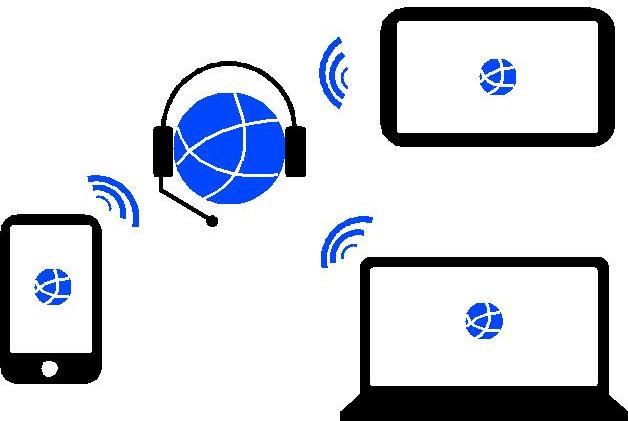
\includegraphics[width=0.5\textwidth]{img/plattformUnabhaengigkeit.jpg}
		\label{plattformUnabhaengigkeit}
	\end{figure}
	
	Durch den offenen Standard ``WebRTC'' ist ``JS VoIP APP'' ist die Applikation auf jedem modernen Gerät benutzbar, das den Standard umsetzt und genug Leistung für Audio- und Videokommunikation bereitstellt.
	
	Durch die einfache Benutzung ist die Applikation auch für nicht versierte Benutzer zugänglich.
	
	Das integrierte Kontaktmanagement kann mit verschiedenen Importformaten umgehen und einfach um weitere Quellen erweitert werden. Dazu gibt es eine Adressbuchschnittstelle.
	
	Die Applikation kann um beliebige Signallingchannel erweitert werden. Somit ist es unter Anderem möglich, die Applikation um signalling über SIP oder XMPP zu erweitern. Dazu gibt es eine Channelschnittstelle.
	
		


% projektorganisation
\chapter{Projektorganisation}

\section{Projektteam}
\subsection*{Tobias Blaser}
\begin{figure}[H]
	
\includegraphics[width=0.3\textwidth]{img/tobias.jpg}
	\centering
	\caption{Tobias Blaser}
	\label{fig:tobias}
\end{figure}

\subsection*{Beat Gutzwiller}
\begin{figure}[H]
	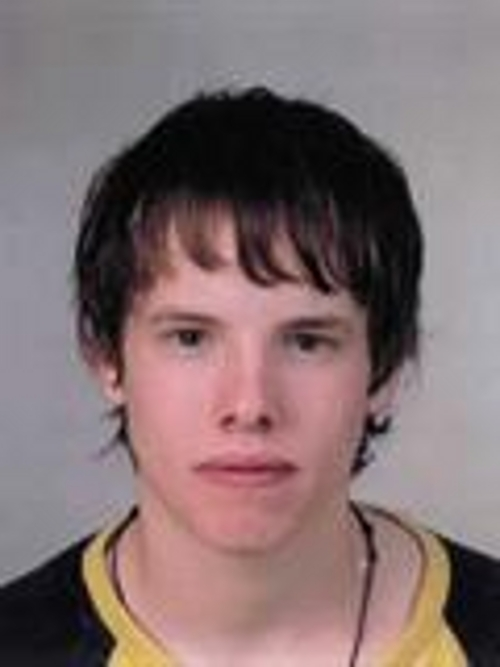
\includegraphics[width=0.3\textwidth]{img/beat.jpg}
	\centering
	\caption{Beat Gutzwiller}
	\label{fig:beat}
\end{figure}

\section{Externe Schnittstellen}
\teacher\ betreut die Semesterarbeit und begleitet das Team durch regelmässige Meetings.


% requirements
\chapter{Allgemeine Beschreibung}

\section{Produkt Perspektive}


\section{Produkt Funktion}


\section{Benutzer Charakteristik}


\section{Einschränkungen}


\section{Annahmen}


\section{Use Cases}

%\section{Use Case Diagramm}
%\includegraphics[width=\textwidth]{use-case-diagram.png}
\subsection{Use Case Übersicht}
\begin{itemize}
	\item Anrufen
	\item Telefonbuch importieren
\end{itemize}

\subsection{Use Case Beschreibungen}

\subsubsection{Anrufen}
Ein Benutzer ruft einen andern Benutzer an. Ist der andere Benutzer erreichbar
und verwendet einen kompatiblen Client (WebRTC), so wird er verbunden.
Am Ende des Telefonates beendet der Benutzer das Telefonat und die Verbindung wird beendet.

Der Benutzer kann vor dem Anruf auswählen, ob er Audio und Video aktivieren möchte. Währen dem Telefonat wird die Auflösung der Verbindungsqualität angepasst.

\subsubsection{Telefonbuch importieren}
Der Benutzer wählt eine Quelle aus und importiert die entsprechenden Daten. Die Telefonbucheinträge werden dem Benutzer nach Quelle getrennt angezeigt sowie in einer Übersicht alle zusammen.

Die Applikation informiert den Benutzer darüber, wie viele Kontakte importiert wurden und ob es Einträge mit ungültigen Daten gibt.

\section{Weitere Anforderungen}

\subsection{Qualitätsmerkmale}
Die Applikation soll intuitiv bedienbar sein und die Video- und Audio-Auflösung
soll abhängig von der Verbindungsqualität skaliert werden.


\subsubsection{Functionality}
\begin{itemize}
	%\item[Korrektheit:] 
	%\item[Angemessenheit:] 
	\item[Interoperabilität:] Die Applikation soll auf existierende Standards setzen und wo eigene Standards nötig sind, diese offen dokumentieren.
	\item[Sicherheit:] Die Audio- und Videokommunikation sowie die Verbindung zum Server soll nach Möglichkeit verschlüsselt erfolgen.
\end{itemize}

%\subsubsection{Efficiency}
%\begin{itemize}
%	\item[Wirtschaftlichkeit:] 
%	\item[Zeitverhalten:] 
%\end{itemize}

\subsubsection{Usability}
\begin{itemize}
	\item[Verständlichkeit:] Die Benutzeroberfläche soll selbsterklärend aufgebaut sein. Knöpfe und Labels sollen sprechend bezeichnet sein.
	%\item[Bedienbarkeit:] 
	\item[Robustheit:] Die Oberfläche soll nicht hängen bleiben bei länger dauernden Operationen und auf Fehler angemessen reagieren.
\end{itemize}

%\subsubsection{Reliability}
%\begin{itemize}
%	\item[Reife:] RC 1
%	\item[Fehlertoleranz:] 
%	\item[Wiederherstellbarkeit:] 
%\end{itemize}

\subsubsection{Portability}
\begin{itemize}
	\item[Anpassbarkeit:] Die Applikation soll so gestaltet werden, das sich die Unterstützung für weitere Technologien einfach hinzufügen lässt.
	\item[Installierbarkeit:] Die Applikation soll auf jedem WebRTC fähigen modernen Browser laufen, der sich an die Standard Darfts hält.
	\item[Austauschbarkeit:] Die Oberfläche soll durch eigene Styles einfach umgestaltet und angepasst werden können.
\end{itemize}

%\subsubsection{Maintainability}
%\begin{itemize}
%	\item[Analysierbarkeit:] 
%\end{itemize}

\subsection{Schnittstellen}

\subsubsection{Signalling-Schnittstelle}
Die Applikation soll als Signalling-Technologie einen offenen Standard (zum
Beispiel SIP oder XAMPP) unterstützen.

\subsubsection{Telefonbuchschnittstelle}
Die Telefonbuchschnittstelle soll offene und verbreitete Standardformate
unterstützen (beispielsweise vCard, CSV, JSON …).


% Risiken
\chapter{Risiken}
	\section{Zusammenfassung}
		Die beiden Hauptrisiken sind die Performance und die Machbarkeit der SIP Anbindung. Zur Verminderung dieser sollen diese Punkte so früh wie möglich untersucht werden.
	
	\section{Ausführliche Risikoanalyse}	
		Siehe Anhang \ref{risiken}


% architektur analyse
\chapter{Domainmodell}

\section{Architekturmodell}
Der logische Aufbau der Software besteht aus vier Schichten:
\begin{figure}[h]
	\centering
	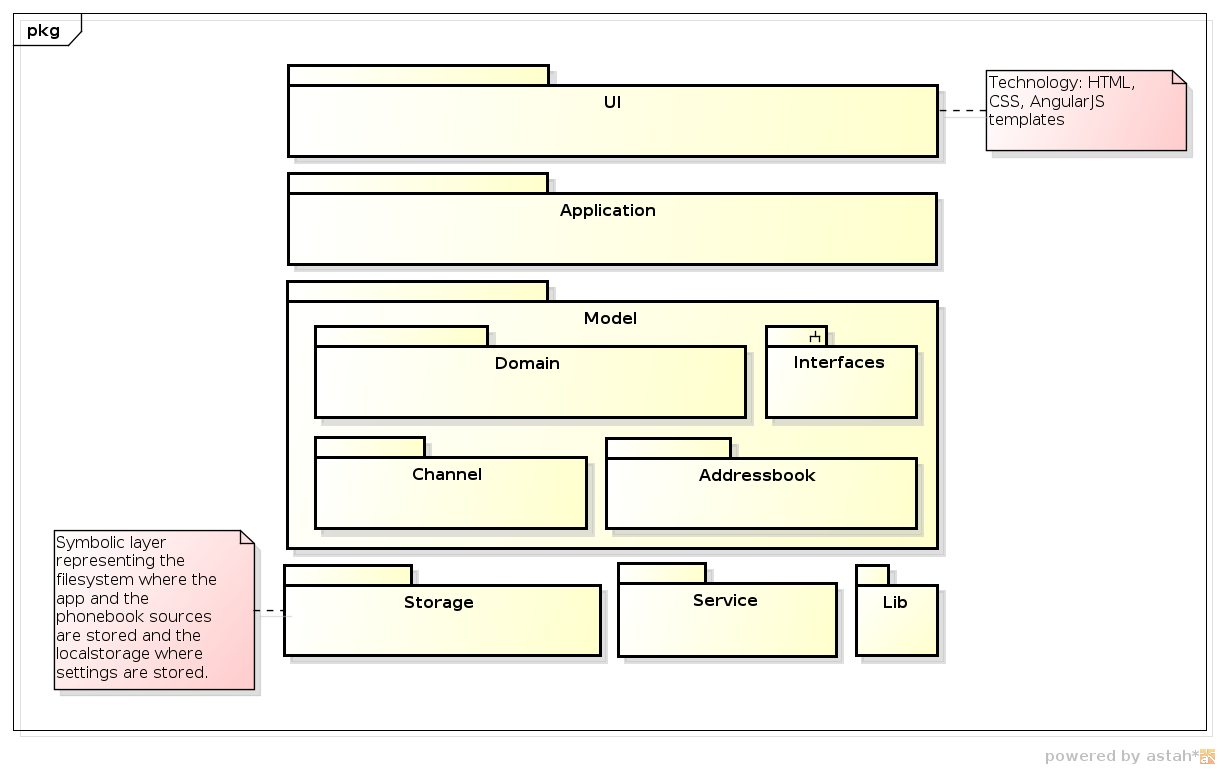
\includegraphics[width=1\textwidth]{img/architecture.png}
	\caption{Architekturdiagramm JS VoIP App}
\end{figure}

\begin{landscape}
\section{Strukturdiagramm}
Im folgenden Diagramm sind die wichtigsten konzeptionellen Klassen und ihre Beziehungen untereinander aufgeführt.
\begin{figure}[h]
	\centering
	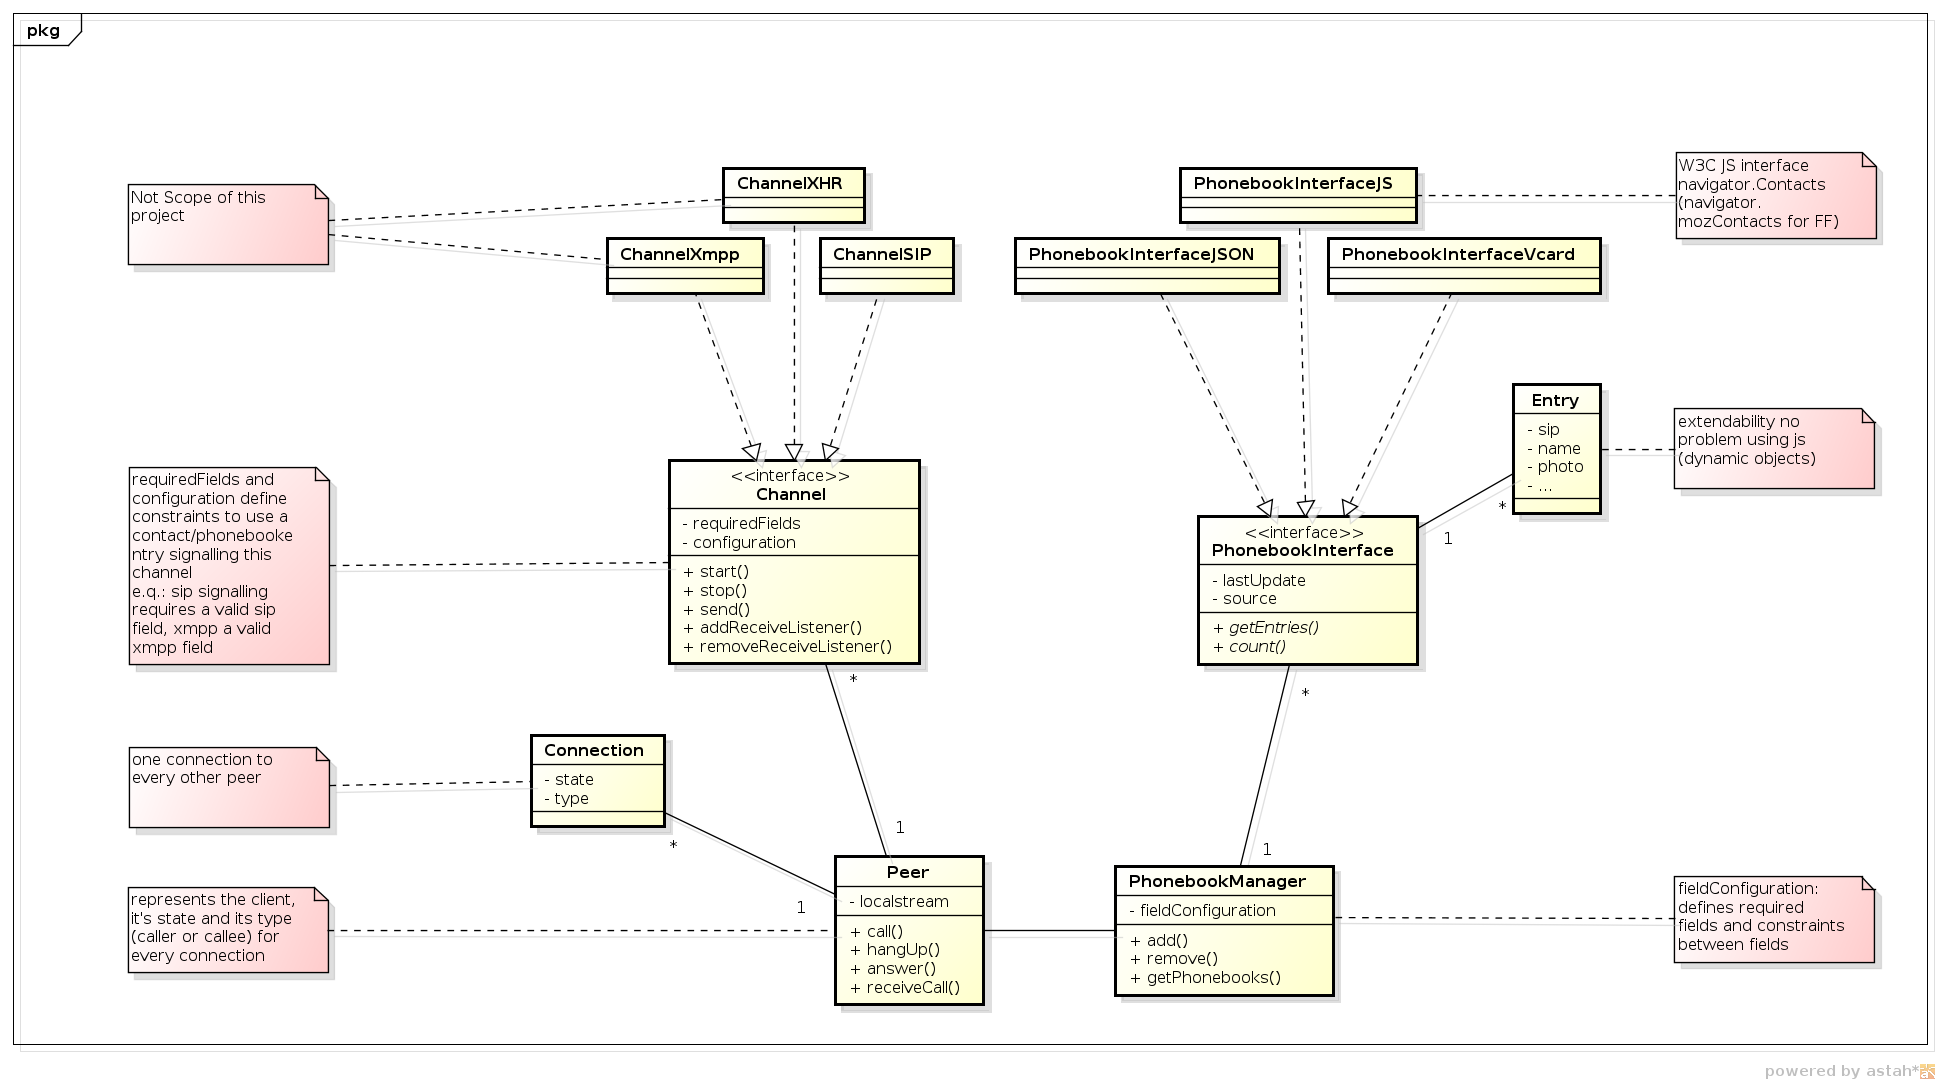
\includegraphics[width=1.2\textwidth]{img/domain.png}
	\caption{Strukturdiagramm JS VoIP App}
\end{figure}
\end{landscape}
\clearpage

\section{Deployment}
Die Applikation wird als ZIP-Datei ausgeliefert oder auf einem Webserver zur Verfügung gestellt. Der Benutzer kann die Datei entpacken und die darin enthaltene HTML Datei mit seinem Browser öffnen.
\begin{figure}[h]
	\centering
	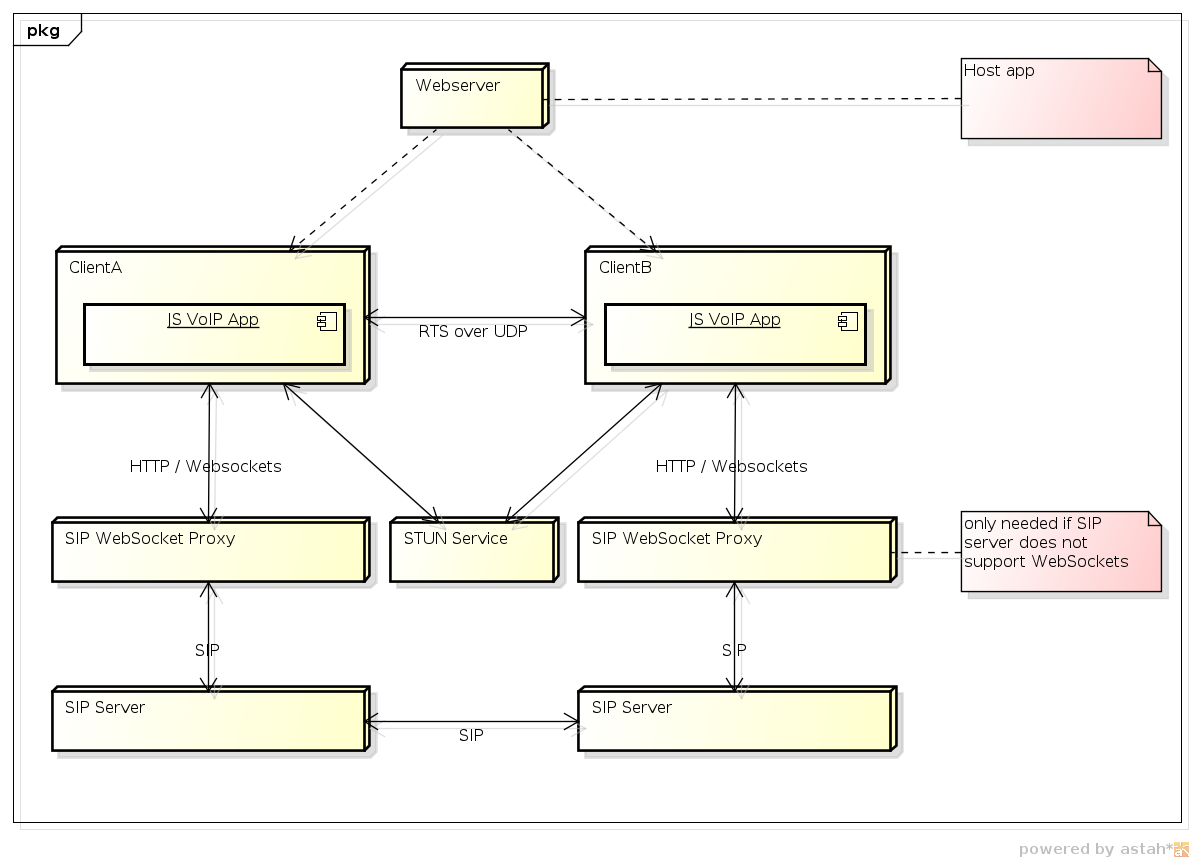
\includegraphics[width=1\textwidth]{img/deployment.png}
	\label{img:deployment}
	\caption{Deploymentdiagramm JS VoIP App}
\end{figure}


% performance analyse
\chapter{Performanceanalyse}
	\section{Zusammenfassung}
		Die Performance hängt sehr stark von der Leistung des Prozessors ab. Videodecodierung und Verschlüsselung verbrauchen in den aktuellen Versionen von Firefox enorm viel Leistung.
		
	\section{Ausführliche Analyse}
		Siehe Anhang \ref{performanceanalyse}
	

% Erkenntnisse
\chapter{Erkenntnisse}
	Die während der Entwicklung der Architekturprototypen und dem Ausbau der Connection gesammelten Erkenntnisse sind hier zusammengetragen:

	\section{Media Streaming}
		\begin{description}
			\item[Verbindungsabbruch] Bricht die Verbindung ab, so bleibt die Video- und Audiowiedergabe stehen, bis die Verbindung wieder da ist und die UDP Pakete wieder ankommen.
		
			\item[Downsampling] Der Mediastream wird automatisch mit Minimalqualität gestartet und abhängig
	 		von Prozessorleistung und Bandbreite hochgefahren, bis zu einer Datenrate von etwa 300MiB/s.
	 		
	 		\item[Resolution Properties] Obwohl die Spezifikation für getUserMedia eine Möglichkeit zur Festlegung der gewünschten Auflösung definiert, ist dies in den Browsern bisher nicht implementiert.
	 		
	 		\item[Audio/Video attach/detach] Hinzufügen und Entfernen von Streams sollte eigentlich möglich sein. Die
	 		Browser implementieren dies bisher jedoch nicht. Gemäss dem Mozilla-Blog soll dieses Feature jedoch demnächst umgesetzt werden.
	 	\end{description}
	 	
	 \section{Peerconnection}
	 	Eine Peer-Connection kann nur durch den Austausch von SDP aufgebaut werden. Innerhalb der SDP werden Parameter für die Peer-Connection
	 	sowie IP und allenfalls Endpunktkandidaten übertragen.
	 	
	 	\begin{description}
			\item[Endpunktkandidaten] Je nach Implementation übertragen die Browser die Endpunktkandidaten (Candidates) einzeln und nicht in einer bestimmten Reihenfolge. Ist die Verbindung noch nicht initialisiert worden, so müssen diese zwischengespeichert werden, bis die Verbindung bereit ist.

			\item[Verschlüsselung] Der übertragene Stream ist standardmässig verschlüsselt. Die Verschlüsselung ist Teil des Standards und kann nicht abgeschaltet werden.
			
			\item[Verbindungsaufbau] Ice Candidates müssen einer RTCPeerConnection attatched werden, bevor eine Offer oder eine Answer generiert wird. Ansonsten hat der andere Endpunkt zu wenig Informationen, um eine Verbindung aufzubauen. Die Ice Candidates sind Proposals für Verbindungsendpunkte (Ports). Die Browser senden einandern mehrere möglich Kombinationen für jede Art von Verbindung (DataChannel, Video, Audio). Anschliessend werden alle Kombinationen probiert, bis eine funktioniert.
	 	\end{description}
	 
	 \section{Filezugriff}
	 	Dateizugriff ist in JavaScript nur über einen User-Event möglich (Upload
	 	Field oder Drag/Drop). Daher ist es nicht möglich, Adressbücher auf die
	 	Festplatte abzulegen und wieder zu öffnen, ohne den User dazu aufzufordern.
	 	
	 
	 \section{Offline-Einschränkungen}
	 	\begin{description}
			\item[Stun Services] Ohne eigener Stun Service ist eine Internet Verbindung zwingend. Für Telefonie in einem abgeschotteten Netz wird ein eigener Stun Service benötigt. Es ist nicht möglich auf die Stun Services zu verzichten und die Adresse manuel zu setzen, weil das Stun Protokoll auch den P2P Verbindungsaufbau übernimmt.
	 	\end{description}
	 		
	 \section{SIP}
	 	\begin{description}
			\item[WebSockets] Obwohl der OpenSource-SIP-Server Kamailio WebSocket als Feature aufführt,
	 		ist die Implementation noch nicht vollständig, sodass SIP-Kommunikation über
	 		WebSockets noch unmöglich ist.
	 	\end{description}
	 		
	\section{Browserunterschiede}
		\begin{description}
			\item[Ice Candidates] Firefox packt die Ice Candidates\footnote{Vorschläge für Ports} direkt in die Session Description ein. Chrome schickt sie einzeln. Da Chrome nicht auf die Reihenfolge achtet kann es passieren, das Ice Candidates vor einer Offer ankommen. Aus diesem Grund müssen ankommende Ice Candidates in einer Queue gebuffert werden, bis eine Offer ankommt.
		
			\item[DataChannel] Firefox unterstützt DataChannel\footnote{P2P-Datenkanal parallel zum Video-
			und Audiostream} bereits vollständig. Chrome unterstützt ihn nur im Modus
			"`reliable: false"'. Setzt man ihn auf "`reliable: true"', kommen die Events
			nicht zuverlässig an.
			
			\item[Media Access] Firefox erlaubt mehrfachen Kameraacces und teilt sich die Kamera auch problemlos mit andern Prozessen. So ist es im Firefox möglich, von einem Tab in einen andern anzurufen. Chrome will die Kamera komplett für sich beanspruchen und wirf eine Fehlermeldung, falls sie bereits von einem Andern Prozess genutzt wird.
			
			\item[Schnittstellenbezeichnung] Die Schnittstellen unterstützen beide Browser erst mit Prefix. Die offizielle Bezeichnung wird noch nicht unterstützt. Adapter.js wurde dafür entwickelt und mappt die offiziellen Schnittstellenbezeichnungen auf die mit Prefix, sodass in der Applikation trotzdem mit den offiziellen gearbeitet werden kann und auch Kompatibilität besteht, sobald die Browser auf die definitiven Schnittstellen umstellen.
	 	\end{description}

% Schluss / Schlussfolgerung
\chapter{Schlussfolgerungen}
	\section{Was wurde erreicht}
	Es ist gelungen, mit JavaScript eine Video-Over-IP Applikation zu entwickeln, die ohne Serverkomponenten auskommt.
	
	Die Applikation benutzt die neuen WebRTC Schnittstellen ``MediaStream"', ``RTCPeerConnection"' und ``RTCDataChannel"'. Daneben werden ``LocalStorage"' für die Speicherung der Kontaktbücher und der Benutzeraccounts sowie ``FileReader"' für den Import der Kontaktbücher verwendet.
	
	Die Benutzeroberfläche wurde responsive gestaltet um auf dem Desktop wie auf Mobilgeräten eine angenehme Benutzung zu ermöglichen.
	
	
	\section{Offene Punkte}
	Internationalisierung, SIP Support, CSV Contactbook Adapter wurden bereits im dritten Viertel des Projektes aus den Featurelist entfernt, da sie tieferer Priorität waren und ein umfangreiches Refactoring der Core-Funktionalität wichtiger war.
	
	Auf eine Authentifizierung beim Channel und entsprechende Mechanismen im QueueServer wurde verzichtet, da es sich nur um eine Referenzimplementation handelt und jeder Channel dies selbst handeln kann.
	
	
	\section{Bugs und technische Probleme}
	Es ist nicht gelungen, SIP als Signalling-Protokoll einzusetzen, da die SIP-Server Websockets erst seit kurzem unterstützen und die Schnittstelle im verwendeten SIP-Server Kamailo noch nicht stabil ist. Websockets sind zwingend notwendig, 
%\chapter{Schlussbericht Jannis}

Durch meinen nachträglichen Wechsel in das Projektteam in der dritten Woche war
es zu Beginn des Projekts etwas anstrengender, da ich in kurzer Zeit sämtliche
Vorarbeiten nachvollziehen musste, um produktiv mitarbeiten zu können.

Es war sehr spannend, neue Web-Technologien zu erforschen, gleichzeitig aber
auch frustrierend, als ich feststellen musste, dass ich SIP über WebSockets
nicht umsetzen konnte. Somit musste ich die Arbeit von zwei Wochen aufgeben.

Es war jedoch sehr toll, dass am Ende alles wie geplant funktioniert hat und die
Applikation selbst als Prototyp sehr gut nutzbar war und fehlerfrei
funktionierte.

Von meinem Teamkollegen und von unserem Betreuer habe ich mich sehr gut
unterstützt gefühlt und würde jederzeit wieder gerne eine Arbeit umsetzen.

%\section{Persönlicher Schlussbericht Tobias Blaser}	
	Persönlich habe ich sehr viel gelernt, vor allem im Bereich JavaScript Architektur und Frameworks. Auch im Bereich CSS habe ich mir einiges an neuem Wissen aneignen können, vor allem was Flexbox und LESS betrifft.
	
	Das Erforschen einer sehr modernen Technologie zog die Vorteile mit sich, das als Zielgruppe nur moderne Browser zum Einatz kommen konnten. Dies hat sich sehr positiv auf die Entwicklung ausgewirkt. Wir konnten modernste CSS Funktionalität und JavaScript Schnittstellen verwenden und mussten uns keine Sorgen um nicht unterstützende Browser machen, was sehr angenehm war.
	
	\subsection{Teamarbeit}		
		Unangenehm war die Unsicherheit zu Begin der Studienarbeit wegen der entzogenen Projektzulassung meines ursprünglichen Partners.
	
		Trotz dieser anfänglichen Unsicherheiten hat die Zusammenarbeit nach dem Teamwechsel sehr gut funktioniert. Wir haben beide sehr engagiert gearbeitet und viel Zeit investiert. Besonders in den letzten Wochen.
		
		Die Teamkoordination war angfangs allerdings nicht immer einfach, da wir an unterschiedlichen Tagen an der SA arbeiteten. Nachdem ich meine Büro-Arbeitstage geschoben hatte, wurde das Zusammenarbeiten wesentlich einfacher.

		Auch die Zusammenarbeit mit Herrn Bläser war sehr angenehm. Wir haben sehr viel Unterstützung und wertvolle Inputs erhalten und Herr Bläser hat ein Code Review der Applikation durchgeführt. Hierfür möchte ich mich an dieser Stelle herzlich bedanken.
			
	
	\subsection{Fazit}		
		Für die knappe Zeit hatten wir uns sehr viel vorgenommen. Trotzdem haben wir es geschafft, sogar noch optionale Features einzubauen.
		
		Das Projekt hat eine Menge Spass gemacht, auch wenn es zwischendurch Moment gab, in denen mich JavaScript durch seine Eigenheiten einiges an Nerven gekostet hat.
	
		Nicht ganz so viel Spass hat das Finishing der Dokumentation gemacht. Vor allem weil durch Abstract, Management Summary, Hauptteil und Anhang viele Themen vier Mal durchgekaut werden mussten um sie in unterschiedlicher Kompaktheit zu produzieren.

		
	
	


\begin{thebibliography}{literatur}
	\bibitem{IETF-JSON-RFC} IETF: 
		"`The application/json Media Type for JavaScript Object Notation (JSON)'', RFC4627 (Stand Juli 2006),
		\hyperlink{http://tools.ietf.org/html/rfc4627}{http://tools.ietf.org/html/rfc4627}, 
		[Abruf am 21.11.13]
	\bibitem{IETF-vCard-RFC} IETF: 
		"`vCard Format Spezifikation'', RFC6350 (Stand August 2011),
		\hyperlink{http://tools.ietf.org/html/rfc6350}{http://tools.ietf.org/html/rfc6350}, 
		[Abruf am 21.11.13]
	\bibitem{MDN-XHR-Cross-Site} Mozilla: 
		"`HTTP access control (CORS)'' 
		\hyperlink{https://developer.mozilla.org/en/docs/HTTP/Access_control_CORS}{https://developer.mozilla.org/en/docs/HTTP/Access/Access\_control\_CORS}, 
		[Abruf am 07.10.13]
	\bibitem{Mozilla-STUN-VM} Mozilla: 
		STUN-VM (Stand: 15.01.13), 
		\hyperlink{https://github.com/mozilla/stun-vm}{https://github.com/mozilla/stun-vm},
		[Abruf am 28.10.13]
	\bibitem{Kamailio-Project} Kamailio SIP Server Project: 
		Kamailio Features (Stand: 18.03.2013), 
		\hyperlink{http://www.kamailio.org/w/features/}{http://www.kamailio.org/w/features/}, 
		[Abruf am 28.10.13]
	\bibitem{IETF-DTLS-RFC} IETF: 
		"`Datagram Transport Layer Security'', RFC5764 (Stand: 2010), 
		\hyperlink{http://tools.ietf.org/html/rfc5764}{tools.ietf.org/html/rfc5764}, 
		[Abruf am 28.10.13]
	\bibitem{AdamRoach-WebRTC-Security} Adam Roach: 
		"`WebRTC: Security and Confidentiality'' (Stand: 07.06.13), 
		\hyperlink{http://sporadicdispatches.blogspot.ch/2013/06/webrtc-security-and-confidentiality.html}{http://sporadicdispatches.blogspot.ch/2013/06/webrtc-security-and-confidentiality.html}, 
		[Abruf am 28.10.13]
	\bibitem{MDN-LocalStorage} Mozilla: 
		"`DOM Storage guide'',
		\hyperlink{https://developer.mozilla.org/en-US/docs/Web/Guide/API/DOM/Storage}{https://developer.mozilla.org/en-US/docs/Web/Guide/API/DOM/Storage},
		[Abruf am 21.10.13]
	\bibitem{IETF-SDP-RFC} IETF:
		"`SDP: Session Description Protocol'' (Stand: Juli 2006),
		\hyperlink{http://tools.ietf.org/html/rfc4566}{http://tools.ietf.org/html/rfc4566},
		[Abruf am 28.10.13]
	\bibitem{IETF-STUN-RFC} IETF:
		"`Session Traversal Utilities for NAT (STUN)'' (Stand Oktober 2008),
		\hyperlink{http://tools.ietf.org/html/rfc5389}{http://tools.ietf.org/html/rfc5389},
		[Abruf am 05.11.13]
	\bibitem{QUnit-API} QUnit: %not use in text
		"`QUnit API Documentation'',
		\hyperlink{http://api.qunitjs.com/}{http://api.qunitjs.com/},
		[Abruf am 30.09.13]
	\bibitem{LESS} LESS:
		"`The dynamic stylesheet language'',
		\hyperlink{http://lesscss.org/\#docs}{http://lesscss.org/\#docs}
		[Abruf am 25.11.13]
	\bibitem{ChrisCoiyer-Flexbox} Chris Coiyer:
		"`http://css-tricks.com/snippets/css/a-guide-to-flexbox/'',
		\hyperlink{http://css-tricks.com/snippets/css/a-guide-to-flexbox/}{http://css-tricks.com/snippets/css/a-guide-to-flexbox/},
		[Abruf am 14.10.13]
	\bibitem{RequireJS-API} RequireJS:
		"`RequireJS API'',
		\hyperlink{http://requirejs.org/docs/api.html}{http://requirejs.org/docs/api.html},
		[Abruf am 28.11.13]
	\bibitem{AngularJS} AngualrJS:
		"`AngularJS API Docs'',
		\hyperlink{http://docs.angularjs.org/api/}{http://docs.angularjs.org/api/},
		[Abruf am 28.11.13]
	\bibitem{html5rocks-WebRTC} HTML5rocks:
		"`http://www.html5rocks.com/en/tutorials/webrtc/basics/'',
		\hyperlink{http://www.html5rocks.com/en/tutorials/webrtc/basics/}{http://www.html5rocks.com/en/tutorials/webrtc/basics/},
		[Abruf am 23.09.13]
	\bibitem{MuazKhan-RTCDataChannel} Muaz Khan:
		"`How to use RTCDataChannel'',
		\hyperlink{https://www.webrtc-experiment.com/docs/how-to-use-rtcdatachannel.html}{https://www.webrtc-experiment.com/docs/how-to-use-rtcdatachannel.html}
		[Abruf am 07.11.13]
\end{thebibliography}


\appendix


% projektplan
\chapter{Risikomanagement}
\label{risiken} 
\section{Risiken}

%Die Spalten werden aufgeteilt auf 0.3 resp. 0.7-fache Textbreite
\noindent
\begin{tabular}{|p{0.3\textwidth} | p{0.7\textwidth} |}
	\hline	
	Risiko-ID & 1 \\
	\hline
	Titel & Implementierungshindernis \\
	Beschreibung & Aufgrund einer nicht bedachten Schwierigkeit verzögert sich die
	Entwicklung des Programms. \\
	max. Schaden	& 10h \\
	Eintrittswahrscheinlichkeit & 0.4 \\
	Gewichteter Schaden	& 4h \\
	Vorbeugung	& Sorgfältige Abklärungen im Vorfeld der Implementierung. \\
	Massnahmen	& Zusätzliche Entwicklungszeit, um das Problem zu lösen. \\
	\hline
\end{tabular}
\hspace{0.5cm}
\newline

\noindent
\begin{tabular}{|p{0.3\textwidth} | p{0.7\textwidth} |}
	\hline	
	Risiko-ID & 2 \\
	\hline
	Titel & Verbindungsverlust \\
	Beschreibung & Kurze Unterbrüche in der Verbindung könnten die ganze Session
	beenden. \\
	max. Schaden	& 8h \\
	Eintrittswahrscheinlichkeit & 0.9 \\
	Gewichteter Schaden	& 7.2h \\
	Vorbeugung	& Einarbeitung in SIP Connection Management. \\
	Massnahmen	& Session bei kleinen Unterbrüchen aufrecht erhalten und einen
	schnellen Reconnect einrichten. \\
	\hline
\end{tabular}
\hspace{0.5cm}
\newline
	
	
\noindent
\begin{tabular}{|p{0.3\textwidth} | p{0.7\textwidth} |}
	\hline	
	Risiko-ID & 3 \\
	\hline
	Titel & Browserperformance \\
	Beschreibung & Video und Audio müssen flüssig wiedergegeben werden. \\
	max. Schaden	& 3h \\
	Eintrittswahrscheinlichkeit & 0.1 \\
	Gewichteter Schaden	& 0.3h \\
	Vorbeugung	& Performance-Tests mit Prototypen. \\
	Massnahmen	& Skalierung der Videoqualität, notfalls Priorisierung auf Audio. \\
	\hline
\end{tabular}
\hspace{0.5cm}
\newline
	
	
\noindent
\begin{tabular}{|p{0.3\textwidth} | p{0.7\textwidth} |}
	\hline	
	Risiko-ID & 4 \\
	\hline
	Titel & Langsame Verbindung \\
	Beschreibung & Bei langsamen Verbindungen kann es zu Problemen in der
	Wiedergabe führen. \\
	max. Schaden	& 8h \\
	Eintrittswahrscheinlichkeit & 0.8 \\
	Gewichteter Schaden	& 6.4h \\
	Vorbeugung	& Performance-Tests mit Prototyp und künstlichem Traffic. \\
	Massnahmen	& Skalierung der Videoqualität, notfalls Priorisierung auf Audio. \\
	\hline
\end{tabular}
\hspace{0.5cm}
\newline
	
	
\noindent
\begin{tabular}{|p{0.3\textwidth} | p{0.7\textwidth} |}
	\hline	
	Risiko-ID & 5 \\
	\hline
	Titel & Konferenzschaltung \\
	Beschreibung & Hohe Teilnehmerzahl führt zu hoher Anzahl Verbindungen. \\
	max. Schaden	& 1h \\
	Eintrittswahrscheinlichkeit & 1.0 \\
	Gewichteter Schaden	& 1h \\
	Vorbeugung	& Performance-Tests mit Prototypen. \\
	Massnahmen	& Maximale Anzahl Teilnehmer festlegen. \\
	\hline
\end{tabular}
\hspace{0.5cm}
\newline

	
\noindent
\begin{tabular}{|p{0.3\textwidth} | p{0.7\textwidth} |}
	\hline	
	Risiko-ID & 6 \\
	\hline
	Titel & Kompetenzmangel SIP \\
	Beschreibung & Erfahrung mit SIP mangelt. Unbekannte Probleme möglich. \\
	max. Schaden	& 14h \\
	Eintrittswahrscheinlichkeit & 0.7 \\
	Gewichteter Schaden	& 9.8h \\
	Vorbeugung	& Frühe Einarbeitung in SIP. \\
	Massnahmen	& Zusätzliche Entwicklungszeit. \\
	\hline
\end{tabular}
\hspace{0.5cm}
\newline


\noindent
\begin{tabular}{|p{0.3\textwidth} | p{0.7\textwidth} |}
	\hline	
	Risiko-ID & 7 \\
	\hline
	Titel & NAT \& Firewall Traversal \\
	Beschreibung & NATs und Firewalls lassen sich nicht ohne weiteres durchdringen.
	\\
	max. Schaden	& 20h \\
	Eintrittswahrscheinlichkeit & 0.25 \\
	Gewichteter Schaden	& 5h \\
	Vorbeugung	& Früh Verbindungstests mit NATs und Firewalls durchführen. \\
	Massnahmen	& Zusätzliche Entwicklungszeit investieren zur Unterstützung von
	Proxyservern und Tunneling-Mechanismen. \\
	\hline
\end{tabular}
\hspace{0.5cm}
\newline


\noindent
\begin{tabular}{|p{0.3\textwidth} | p{0.7\textwidth} |}
	\hline	
	Risiko-ID & 8 \\
	\hline
	Titel & Verschlüsselte Verbindung \\
	Beschreibung & Das Verschlüsseln der P2P-Verbindung und des Server-Connects
	gestalten sich schwieriger als gedacht. \\
	max. Schaden	& 16h \\
	Eintrittswahrscheinlichkeit & 0.5 \\
	Gewichteter Schaden	& 8h \\
	Vorbeugung	& Früh Möglichkeiten zur Verschlüsselung und deren
	Implementierungsaufwand analysieren. \\
	Massnahmen	& Zusätzliche Entwicklungszeit investieren zur Umsetzung des
	Verschlüsselungsmechanismus. \\
	\hline
\end{tabular}
\hspace{0.5cm}
\newline


\noindent
\begin{tabular}{|p{0.3\textwidth} | p{0.7\textwidth} |}
	\hline
	Risiko-ID & 9 \\
	\hline
	Titel & Social Risks \\
	Beschreibung & Die Projektmitglieder sind aufgrund anderer Projekte zu stark
	absorbiert und können zu wenig Zeit für das Projekt aufwenden. \\
	max. Schaden & 25h \\
	Eintrittswahrscheinlichkeit & 0.25 \\
	Gewichteter Schaden	& 6h \\
	Vorbeugung	& Externe Projekte in der Iterationsplanung berücksichtigen. \\
	Massnahmen	& Projektmitglieder opfern ihre Freizeit und trinken mehr Red Bull.
	\\
	\hline
\end{tabular}
\hspace{0.5cm}
\newline


\section{Umgang mit Risiken}
Um die Riskien möglichst kalkulierbar zu halten, ist es für dieses Projekt
entscheidend, möglichst früh Evaluationen durchzuführen. Besonders die frühe Einarbeitung in SIP sowie die Bereitstellung eines ersten
Prototypen mit SIP-Verbindung muss gewährleistet werden. Sobald Prototypen
vorhanden sind, müssen erste Performance-Test durchgeführt werden. Weiterhin
sollten die Risiken laufend neu beurteilt werden.

\chapter{Projektplan}
Die einzelnen Arbeitspakete werden mithilfe des Projektverwaltungstools Redmine
organisiert. Für die Betreuer wurde ein eigener Zugang zum Redmine-Projekt eingerichtet.

%\section{Gastzugang Redmine}
%http://152.96.192.44/redmine \\
%Zugang: guest / zurich2Rapperswil \\

	\section{Milestones}
		\subsubsection{Elaboration I2 - MS core prototypes}
			\begin{itemize}
				\item Prototypen der Kernkomponenten, insbesondere der Komponenten mit hohen Risiken
					\begin{itemize}
						\item WebRTC P2P Communication Prototype
						\item SIP Server Connection Prototype
						\item Addressbook Interface Implementation Prototype
						\item Channel Interface Implementation Prototype (XHR Simple Queue Server)
					\end{itemize}
				\item Risikoanalyse
				\item Architekturanalyse
			\end{itemize}
			
		\subsubsection{Construction I2 - MS core functionality}
			\begin{itemize}
				\item Implementation der Kernkomponenten (Prototyp-Komponenten-Elaboration)
					\begin{itemize}
						\item P2P Communication
						\item Channel Reference-Implementation
						\item Addressbook Reference-Implementation
					\end{itemize}
				\item Zwischenstand Projektdokumentation
			\end{itemize}
			
		\subsubsection{Construction I4 - MS final app}
			\begin{itemize}
				\item Implementation der Advanced Komponenten
					\begin{itemize}
						\item Media Scaling
						\item Scallable User Interface
					\end{itemize}
				\item Projektdokumentation
			\end{itemize}
		
		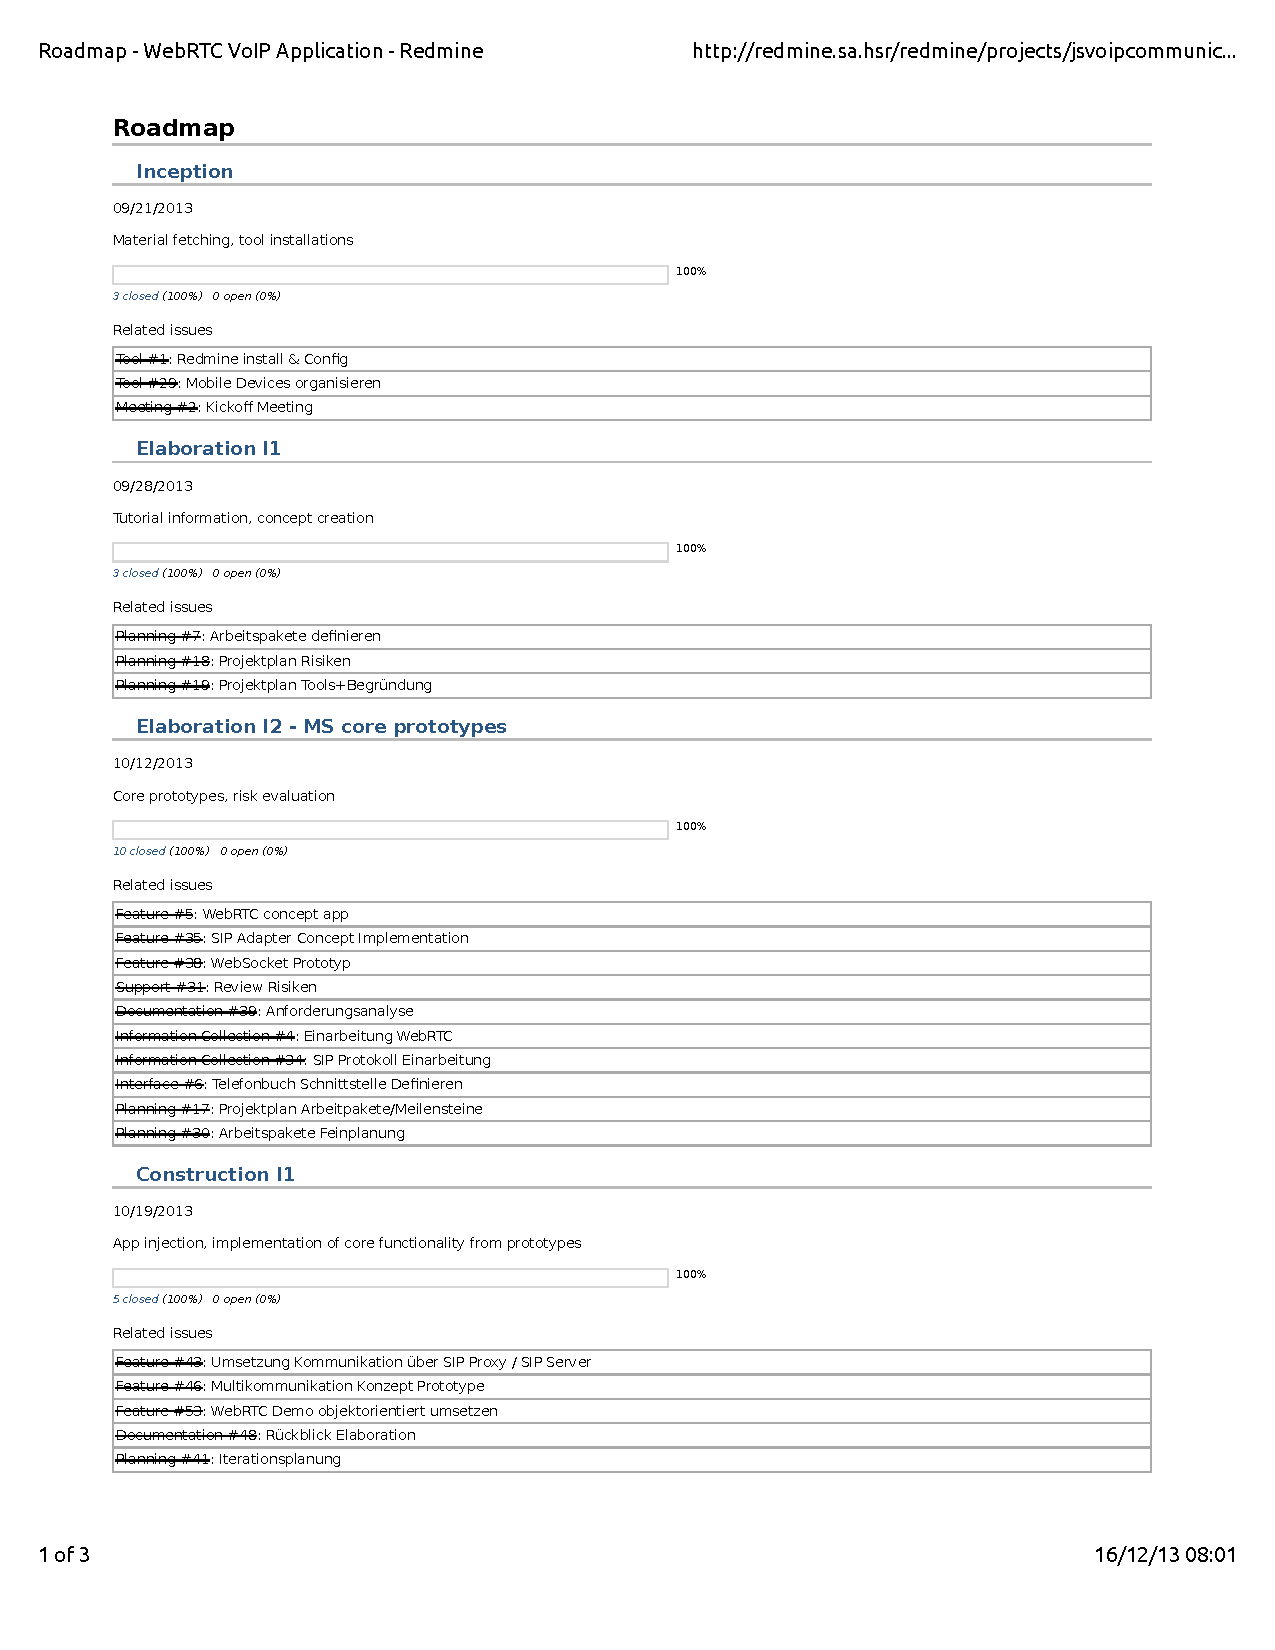
\includepdf[pages=-]{../projektplan/media/roadmap.pdf}
		\begin{landscape}
			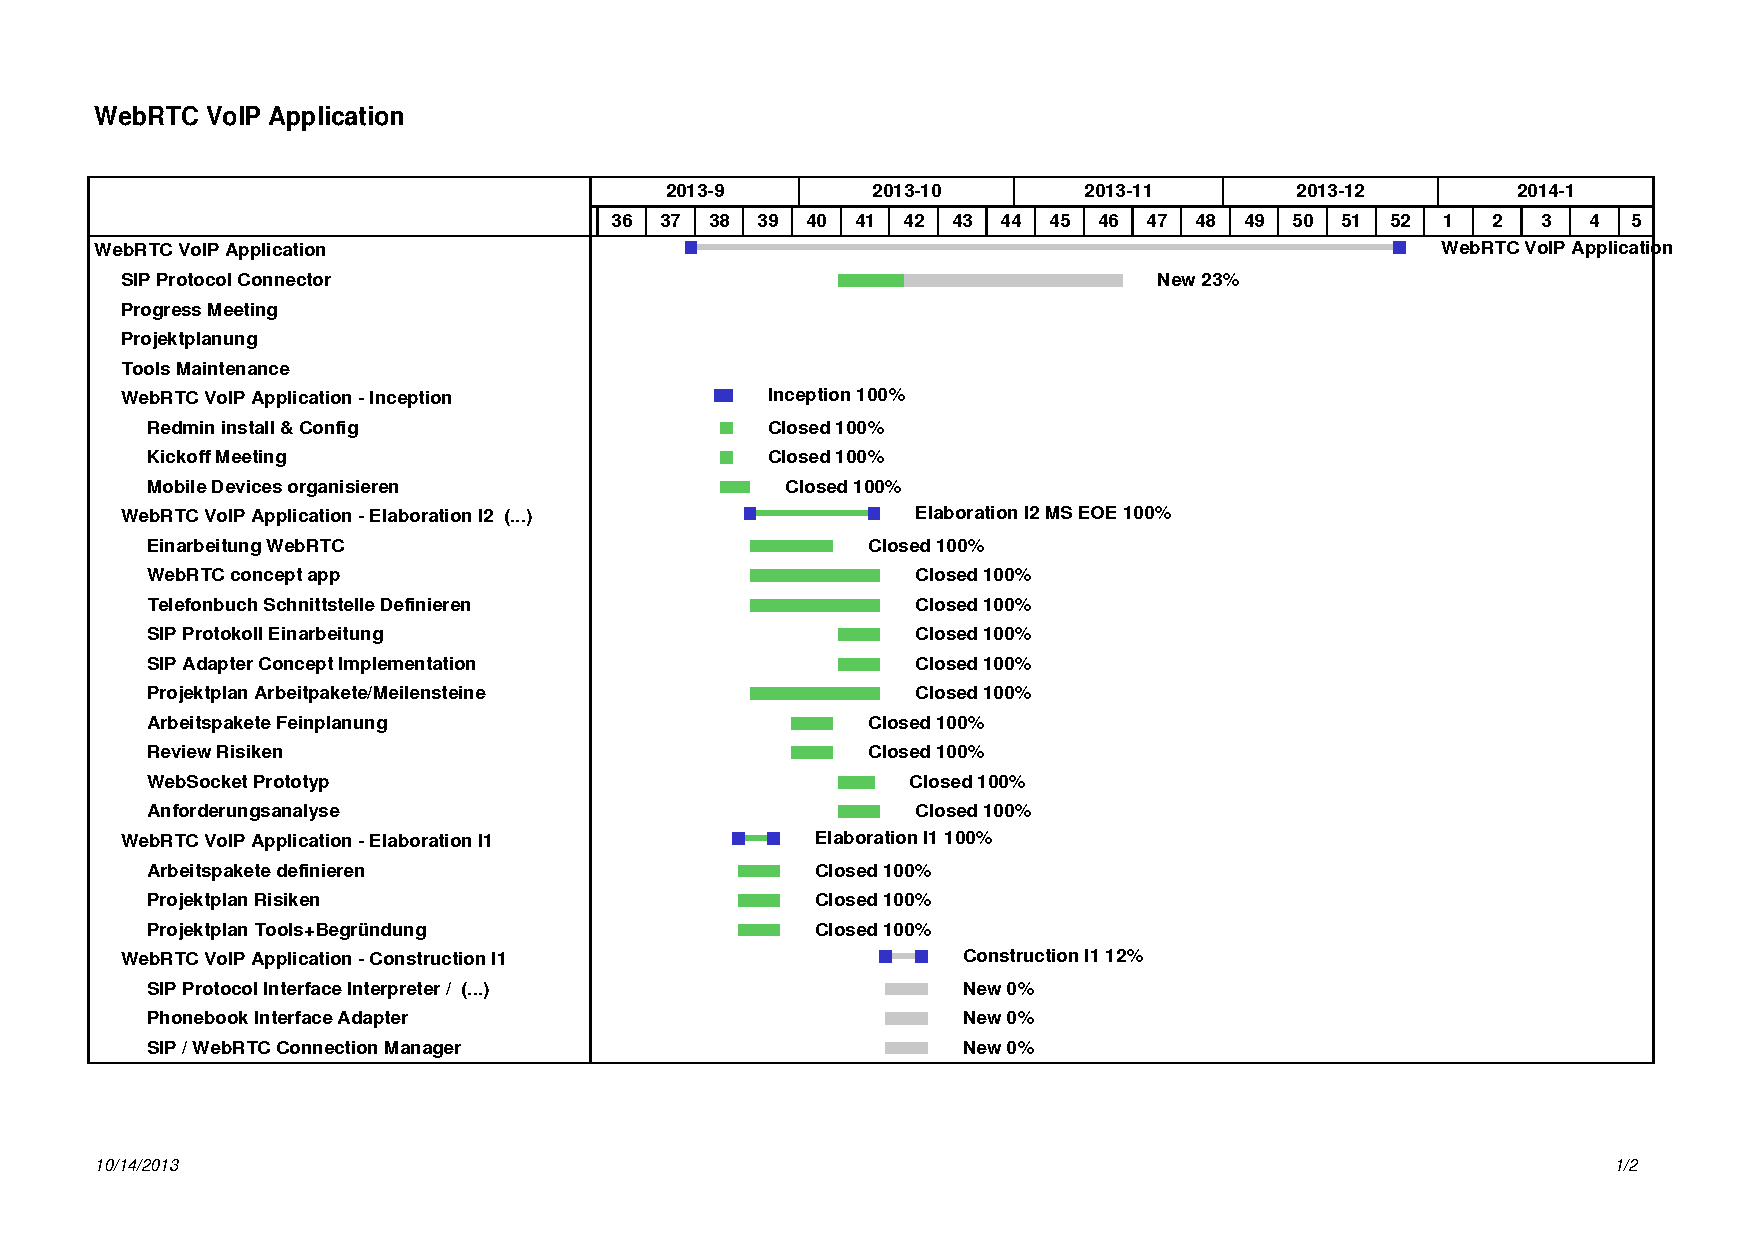
\includepdf[pages=1]{../projektplan/media/jsvoipcommunication-gantt.pdf}
		\end{landscape}
		\begin{landscape}
			\includepdf[pages=2]{../projektplan/media/jsvoipcommunication-gantt.pdf}
		\end{landscape}
		\begin{landscape}
			\includepdf[pages=3]{../projektplan/media/jsvoipcommunication-gantt.pdf}
		\end{landscape}
		
		
	\section{Aufgewendete Zeit}
		\begin{figure}[H]
			\centering
			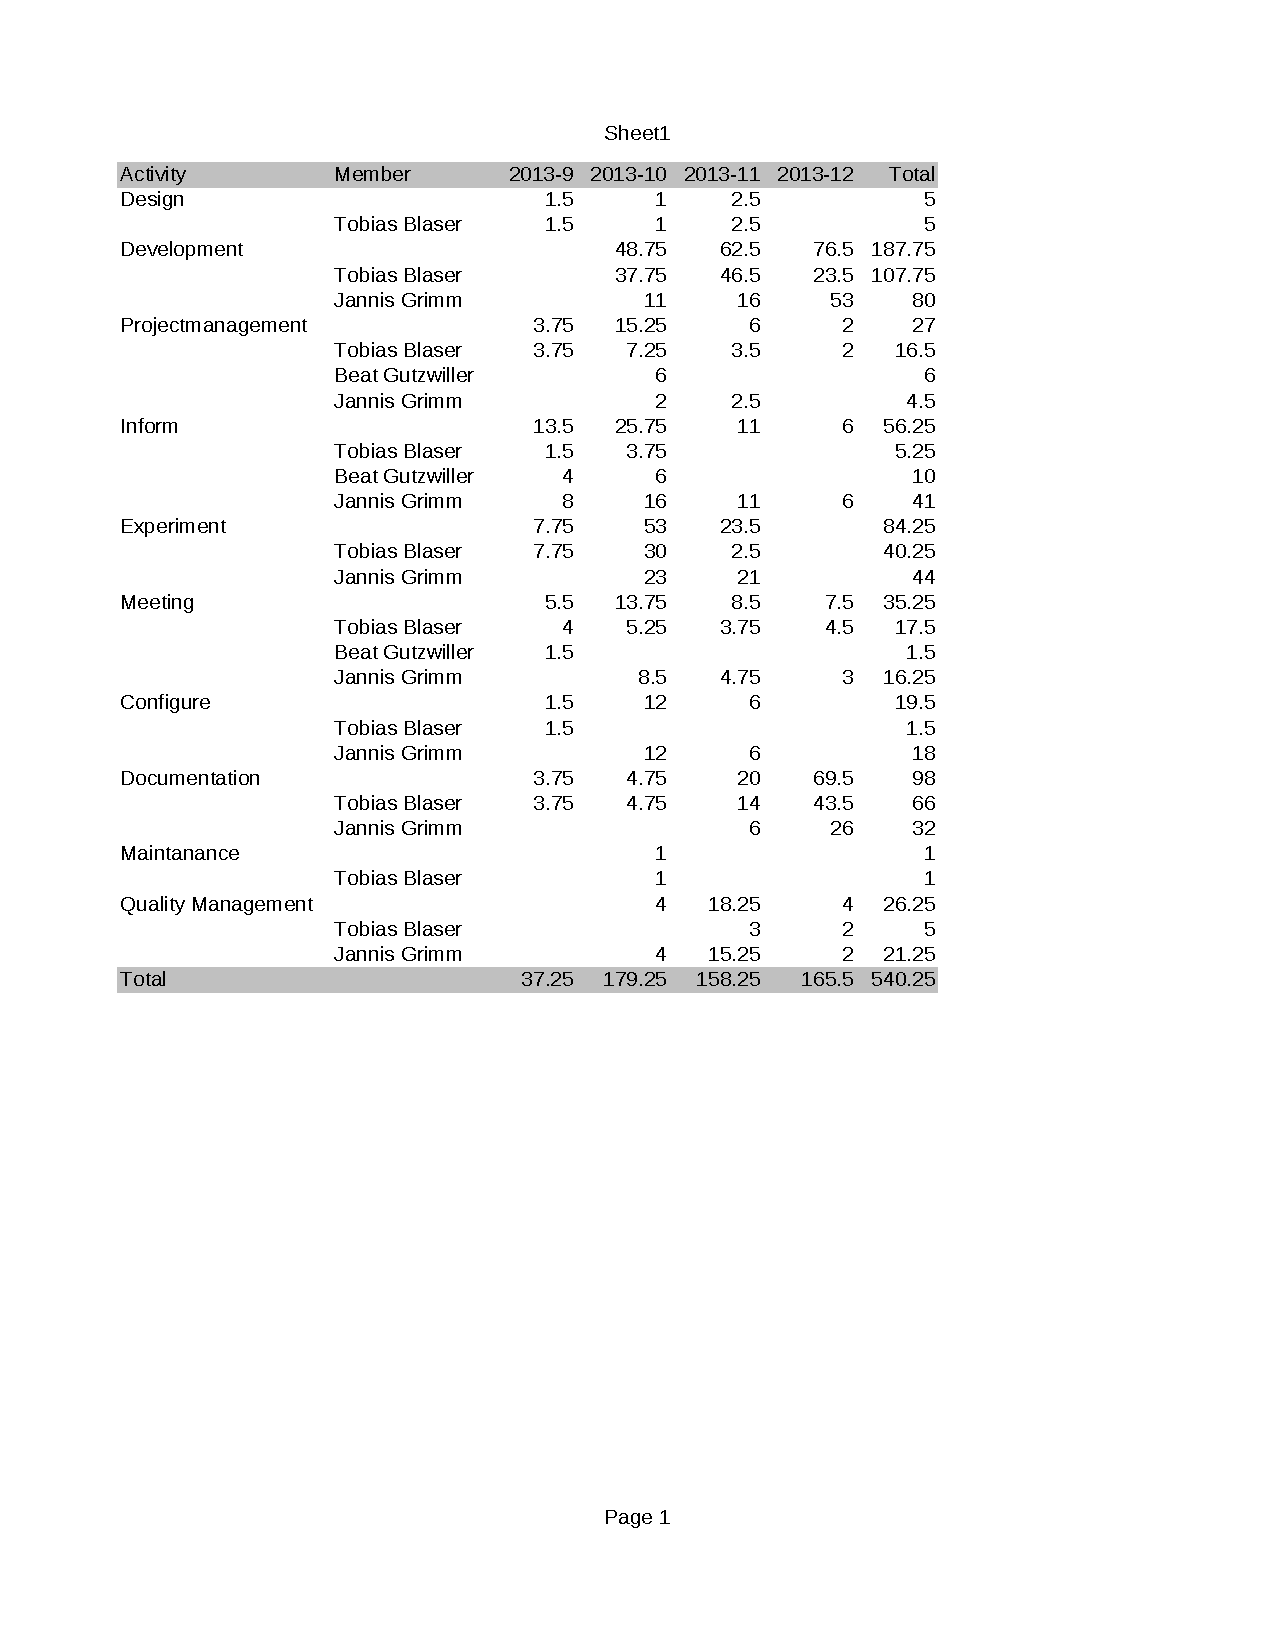
\includegraphics[trim=1.75cm 10cm 5.5cm 2.5cm, clip=true,page=1,width=\textwidth]{../projektplan/media/timelog.pdf}
		\end{figure}
\chapter{Infrastruktur}

\section{Hardware}
\begin{itemize}
	\setlength{\itemsep}{-\parsep}
	\item Persönliche Entwicklungsgeräte für jedes Teammitglied, bevorzugt Laptop (eigene Geräte)
	\item Zugewiesene Arbeitsplätze im Zimmer 1.262
	\item Mobile Devices mit WebRTC fähigem Browser
	\item Virtual Server für Projektmanagement
	\item SIP Service (z.B. sipcall.ch) oder SIP Server
\end{itemize}

\section{Tools}
\subsection{Projektmanagement}
Das Projektmanagementtool Redmine bietet sich aus verschiedenen Gründen an:
\begin{itemize}
	\setlength{\itemsep}{-\parsep}
	\item Redmine ist bekannt vom SE2 Projekt.
	\item Redmine lässt sich auf den Virtual Servern der HSR leicht installieren.
	\item Redmine bietet den benötigten Funktionumfang und ist einfach zu bedienen.
	\item Redmine bietet Git Repository Integration falls dies gewünscht ist.
\end{itemize}


\subsection{Versionsverwaltung}
\subsubsection{Git}
Git ist ein bewährtes Versionsverwaltungstool, bietet den Vorteil von lokalen Repositories, ist sehr schlank und bringt eine gute Merge-Automatik mit.

\subsubsection{GitHub}
Mit GitHub besitzen die Studenten durch andere Projekte bereits Erfahrung. Als Studenten haben sie Zugriff auf kostenlose ``Private-Repositories''. Zudem Bietet GitHub noch zusätzliche Funktionen wie Wiki, RST und MD Viewer sowie Repository Zugriff und Dateibearbeitung über Webinterface.

\subsubsection{Backup}
Ein zusätzliches Backup ist nicht notwendig, da durch die Versionierung mit Git die komplette Versionshistorie bei jedem Teilnehmer vorhanden ist. Somit ist das gesammte Projekt dreifach abgelegt (bei den Entwicklern sowie bei GitHub).


\subsection{Dokumentation}
\subsubsection{Für grosse Dokumentationen und Abgabedokumente: \LaTeX}
\LaTeX ist perfekt geeignet für grosse, gemeinsam zu erarbeitende Dokumente, weil die Source-Dateien über Git versioniert und gemergt werden können und wenig Platz verbrauchen. Zudem besteht ein sehr kleines Risiko auf Dokumentenverlust bzw. Dokumentenfehler durch die Software, weil \LaTeX die Source-Dateien gar nicht verändert im Unterschied zu einer Office Applikation.

\subsubsection{Für Notizen \& Meetingsprotokolle: Restructured Text (rst), txt, Markdown (md)}
Für Notizen und kleine Dokumente reichen RST, TXT oder MD vollständig aus. Sie sind schlank, bieten nur das notwendigste, können versioniert und gemergt werden weil es nur Textfiles sind und werden von "GitHub Document Preview" unterstützt.

\subsubsection{Für Diagramme, Skizzen: Libreoffice Draw (Opendocument)}
Wo es nicht anders geht wird Opendocument eingesetzt. Dabei wird berücksichtigt, dass es über Git nicht inkrementell versioniert und nicht gemergt werden kann.


\subsection{Modelling}
Als Modelling Tool wird Astah gewählt, weil es das beste den Studenten bekannte Tool ist.
Es deckt den geforderten Funktionsumfang grosszügig ab und bietet Image und PDF Export.

\subsection{UI Drafting}
\begin{itemize}
	\setlength{\itemsep}{-\parsep}
	\item Balsamiq Mockup für UI Drafts
	\item ev. Libreoffice Draw für UI Design Finals
\end{itemize}


\subsection{Frameworks}
\subsubsection{Adapter.js}
Adapter.js abstrahiert die verschiedenen Browserschnittstellen von WebRTC und vereinfacht die Entwicklung. Zudem muss bei einer Schnittstellenanpassung browserseitig nur der Adapter aktualisiert werden und nichts an der App geändert werden.

\subsubsection{Ember.js}
Ember.js ist ein bekanntes MVC und Templating Framework, das eine saubere Trennung von Logik und Darstellung ermöglicht. Ember.js bindet darüber hinaus Properties im Template direkt an Objektproperties, wodurch in vielen Fällen eigene Observerimplementierungen überflüssig sind.

\subsubsection{jQuery}
jQuery als eine der besten Javascript Bibliotheken bietet sehr einfache Elementselektoren und viele Funktionen, die das Entwickeln vereinfachen.


\subsection{Testing}
Testing Framework Anforderungen:
\begin{itemize}
	\setlength{\itemsep}{-\parsep}
	\item Testing mit realem Browser, Browsersimulationen unterstützen vermutlich WebRTC noch nicht
	\item Einfach einzubinden
	\item Einfach zu erweitern
	\item Bekannte Benutzung mit Tests und Asserts
	\item Möglichkeit zur Anbindung eines Build Tools
\end{itemize}

\subsubsection{JsUnit}
JsUnit arbeitet mit einem realen Browser, ist einfach handzuhaben und bietet typische Assert-Syntax.


\subsection{Building}
Ein Build Server wie Ant ist nicht nötig für dieses Projekt. JsUnit bietet zwar eine Anbindungsmöglichkeit. Für unsern Anwendungsfall und die nicht sehr komplexe Tool-Umgebung lohnt sich der Aufwand eines Build Servers jedoch nicht.


\subsection{Entwicklungsumgebung}
Jeder Entwickler verwendet seine eigene bevorzugte Entwicklungsumgebung.


\subsection{RunTime Environment}
Als RunTime Environment wird ein WebRTC kompatibler Browser (Firefox, Chrome(ium)) benötigt.




% ui
\chapter{User Interface}

\section{User Interface Draft 1}
	\label{uiDrafts} 

	\begin{figure}[H]
		\centering
		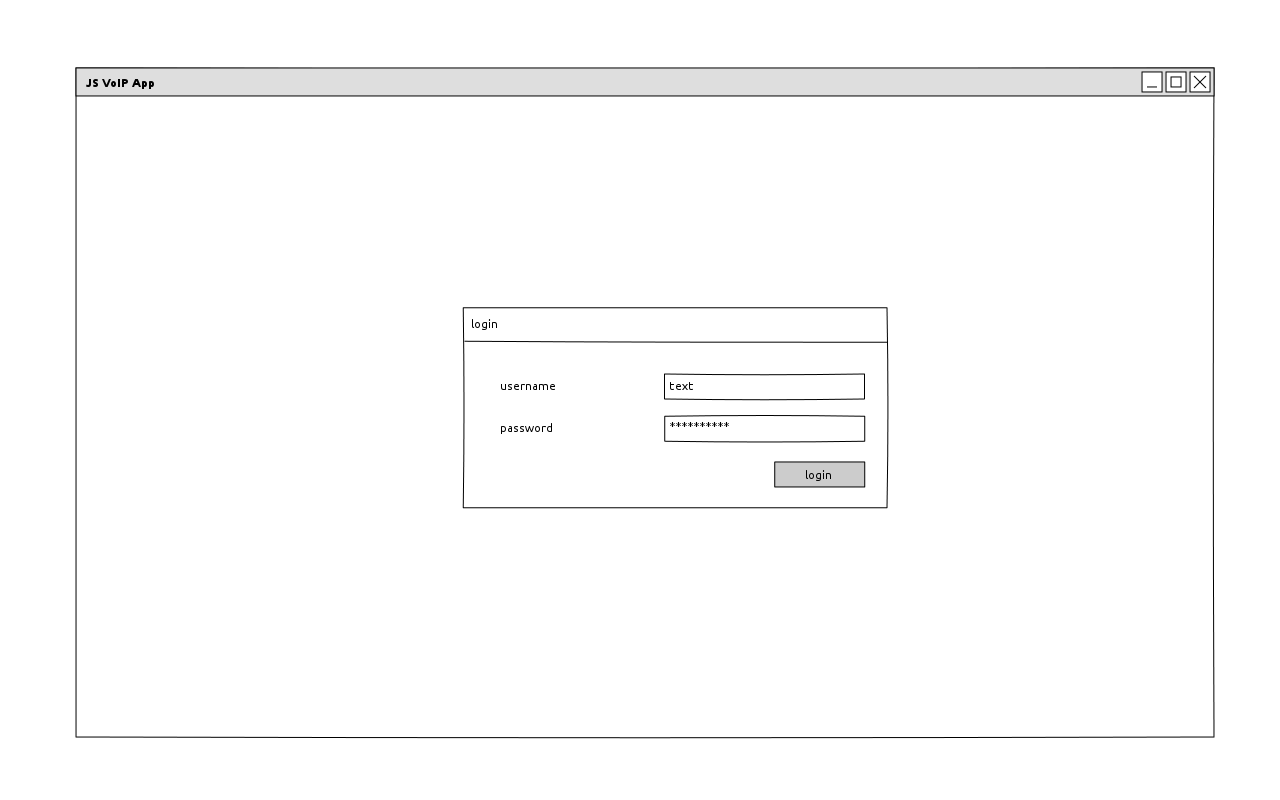
\includegraphics[height=0.3\textheight]{../ui/img/uiDraft1/login_page.png}
		\caption[Login screen draft1]{Über den Login Screen loggen sich Benutzer ein.}
		\label{login screen}
	\end{figure}
	\begin{figure}[H]
		\centering
		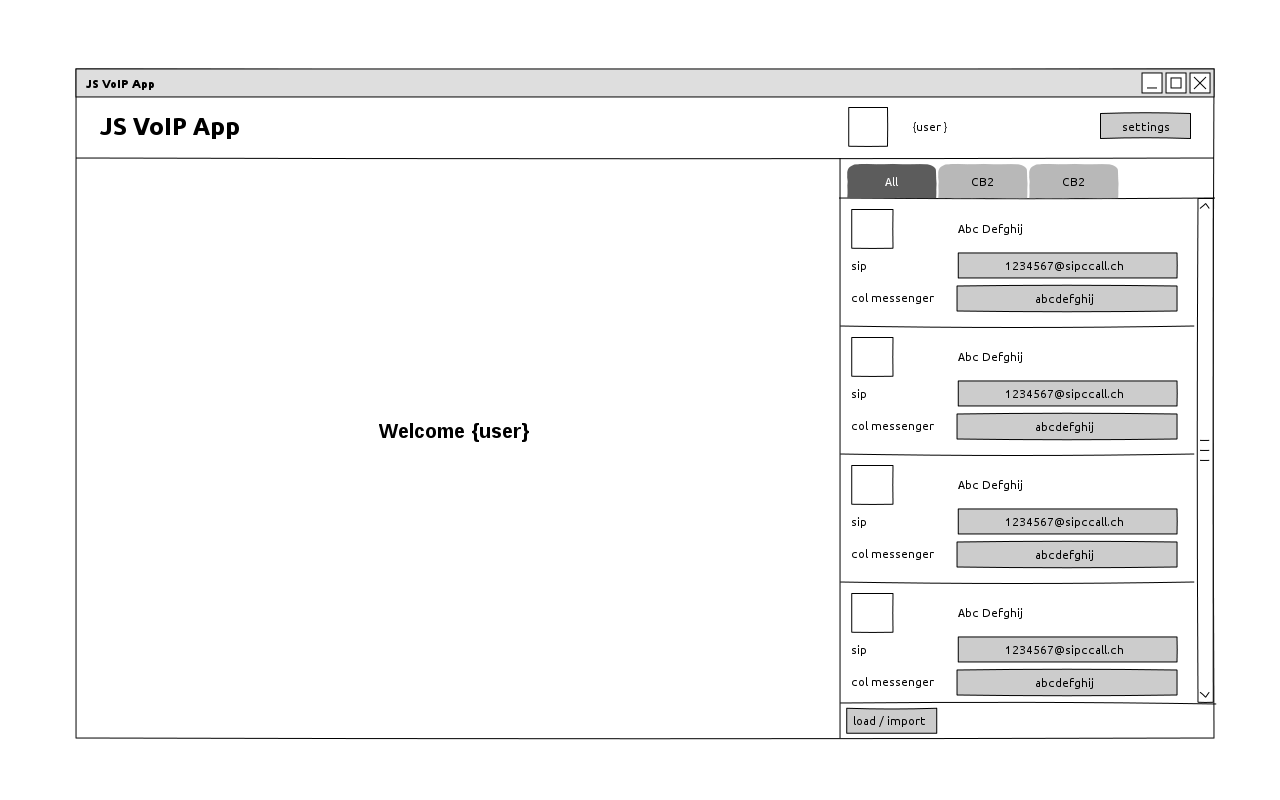
\includegraphics[height=0.3\textheight]{../ui/img/uiDraft1/main_view.png}
		\caption[Main screen draft1]{In der Hauptansicht hat der Benutzer Zugriff auf das Adressbuch.}
		\label{main screen}
	\end{figure}
	\begin{figure}[H]
		\centering
		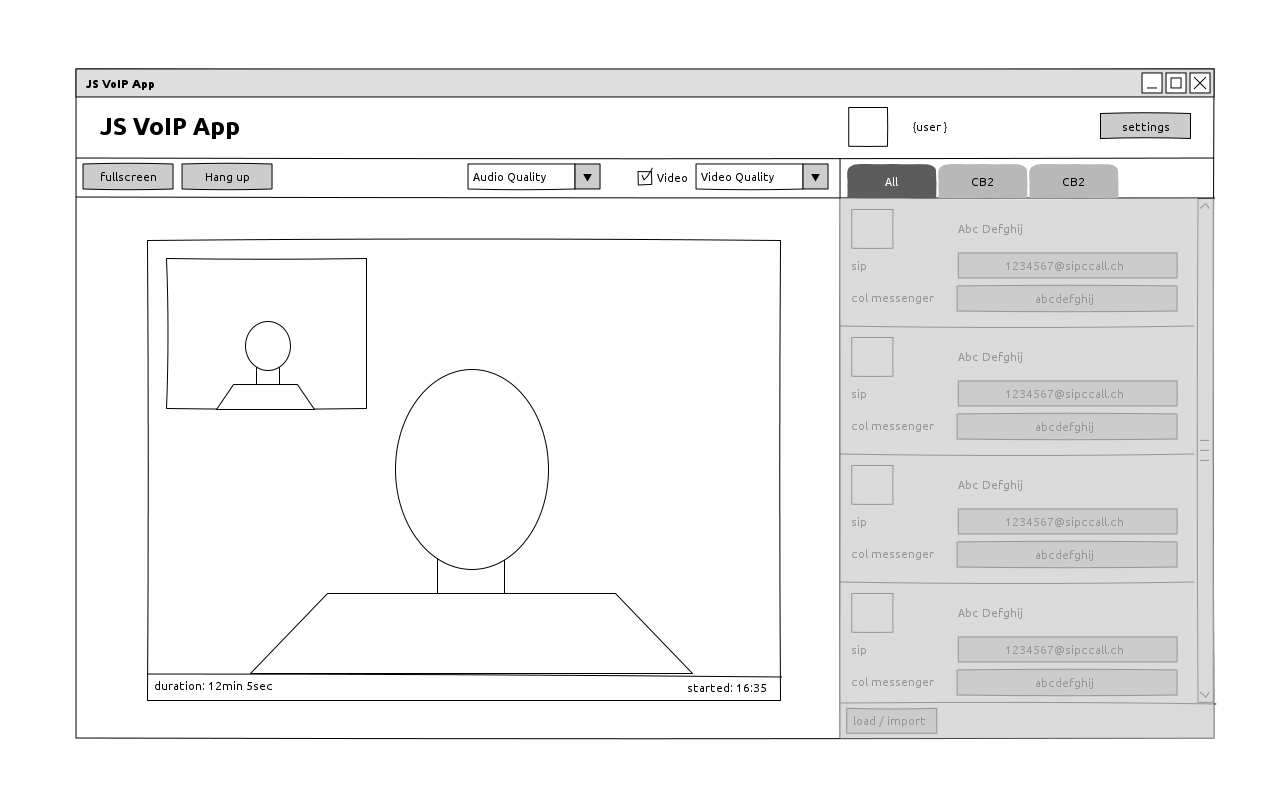
\includegraphics[height=0.4\textheight]{../ui/img/uiDraft1/call_view.png}
		\caption[Phone screen draft1]{Ruft der Benutzer einen Kontakt an, so wird das Video in der Hauptansicht eingeblendet und die Kontakte werden inaktiv.}
		\label{call screen}
	\end{figure}
	\begin{figure}[H]
		\centering
		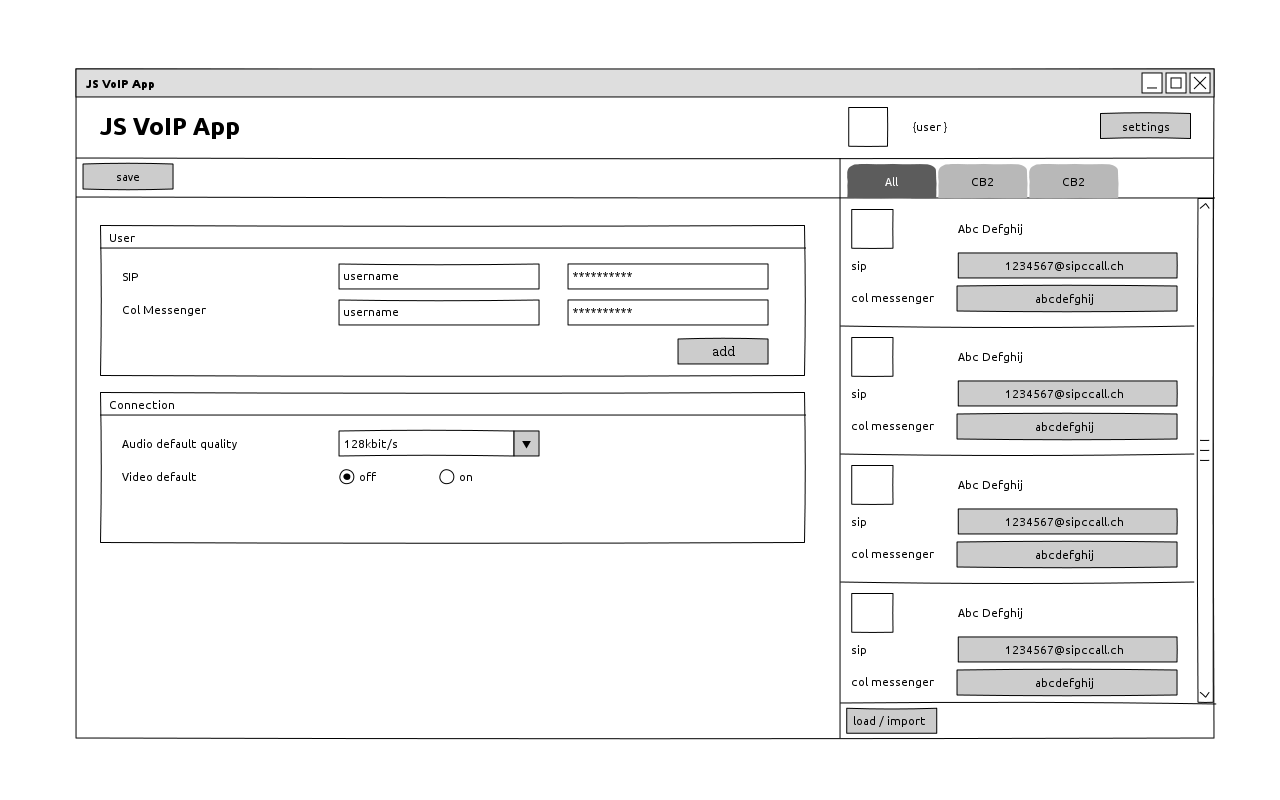
\includegraphics[height=0.4\textheight]{../ui/img/uiDraft1/settings_view.png}
		\caption[Settings screen draft1]{Über die Settings kann der Bentzer Einstellungen verändern.}
		\label{settings screen}
	\end{figure}
	
	
\section{User Interface Draft 2}
	Das UI2 folgt dem Prinzip ``Mobile First"'.
	\begin{figure}[H]
		\centering
		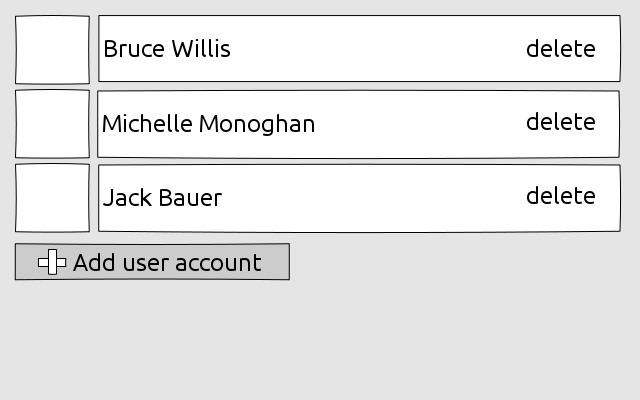
\includegraphics[height=0.35\textheight]{../ui/img/uiDraft2/UserView-selectUser.png}
		\caption[Accound screen draft2]{Benutzer Verwaltung und Login Screen. Durch klick auf einen Benutzer kann sich der Benutzer mit dessen Konto anmelden.}
		\label{login screen}
	\end{figure}
	\begin{figure}[H]
		\centering
		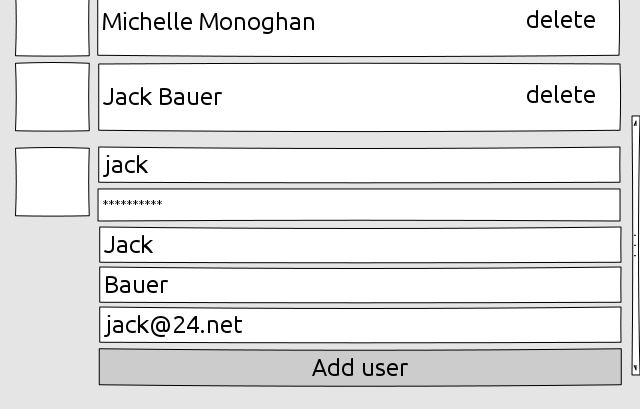
\includegraphics[height=0.35\textheight]{../ui/img/uiDraft2/UserView-addUser.png}
		\caption[Account management Screen draft2]{Die Benutzerverwaltung erlaubt es dem benutzer auch gleich einen neuen Bentzer zu erfassen.}
		\label{user management screen}
	\end{figure}
		\begin{figure}[H]
		\centering
		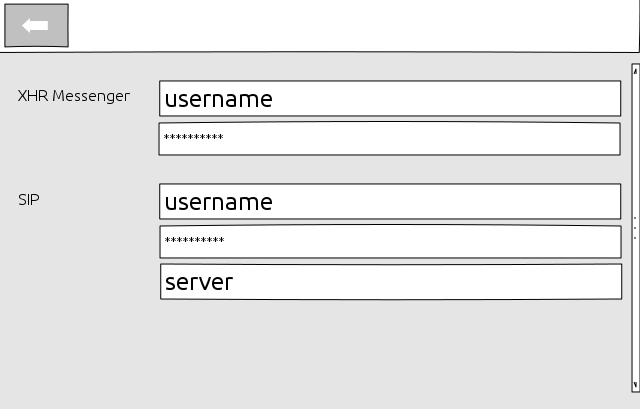
\includegraphics[height=0.4\textheight]{../ui/img/uiDraft2/UserView-addChannel.png}
		\caption[Channel edit screen draft2]{Die Bentzerverwaltung ermöglicht dem Benutzer das verwalten der verfügbaren Channel Accounts.}
		\label{user management screen}
	\end{figure}
	\begin{figure}[H]
		\centering
		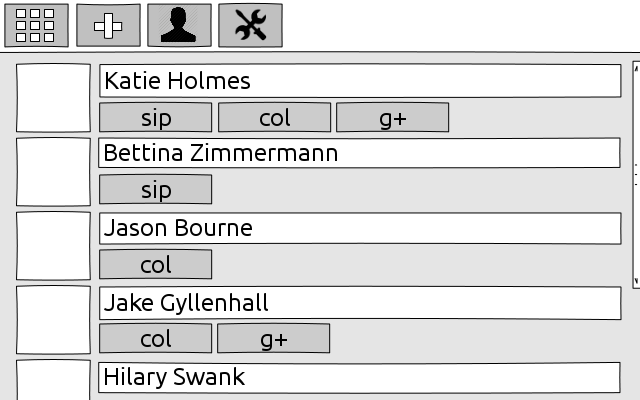
\includegraphics[height=0.4\textheight]{../ui/img/uiDraft2/ContactbookView.png}
		\caption[Contactbook screen draft2]{Adressbuch: Von hier aus ruft der Benutzer seine Kontakte an. Die verschiedenen Adressbücher sind über das Listensymbol erreichbar.}
		\label{contactbook screen}
	\end{figure}
	\begin{figure}[H]
		\centering
		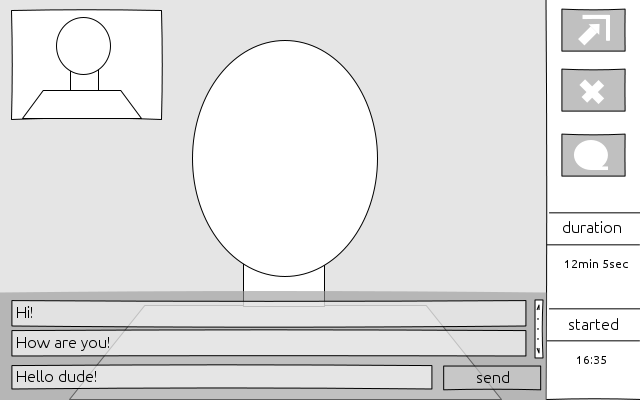
\includegraphics[height=0.4\textheight]{../ui/img/uiDraft2/PhoneViewWithMessenger.png}
		\caption[Call screen draft2]{Phone View: Nebst dem Video sieht der Benutzer elementare Informationen über den Anruf.}
		\label{settings screen}
	\end{figure}
	\begin{figure}[H]
		\centering
		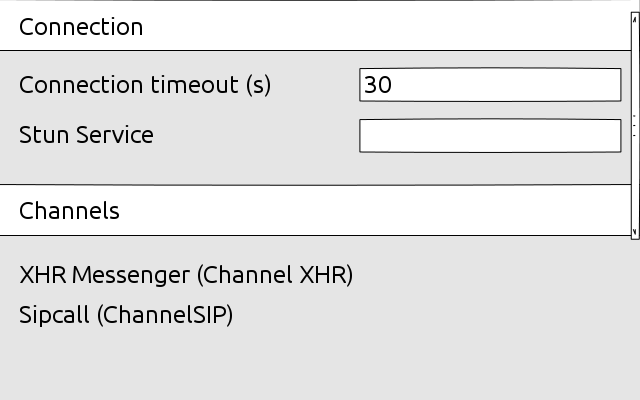
\includegraphics[height=0.4\textheight]{../ui/img/uiDraft2/SettingsView.png}
		\caption[Settings screen draft2]{In den Settings kann der Benutzer Konfiguration und Channels einsehen.}
		\label{settings screen}
	\end{figure}
	
\section{Finales User Interface}
	\begin{figure}[H]
		\centering
		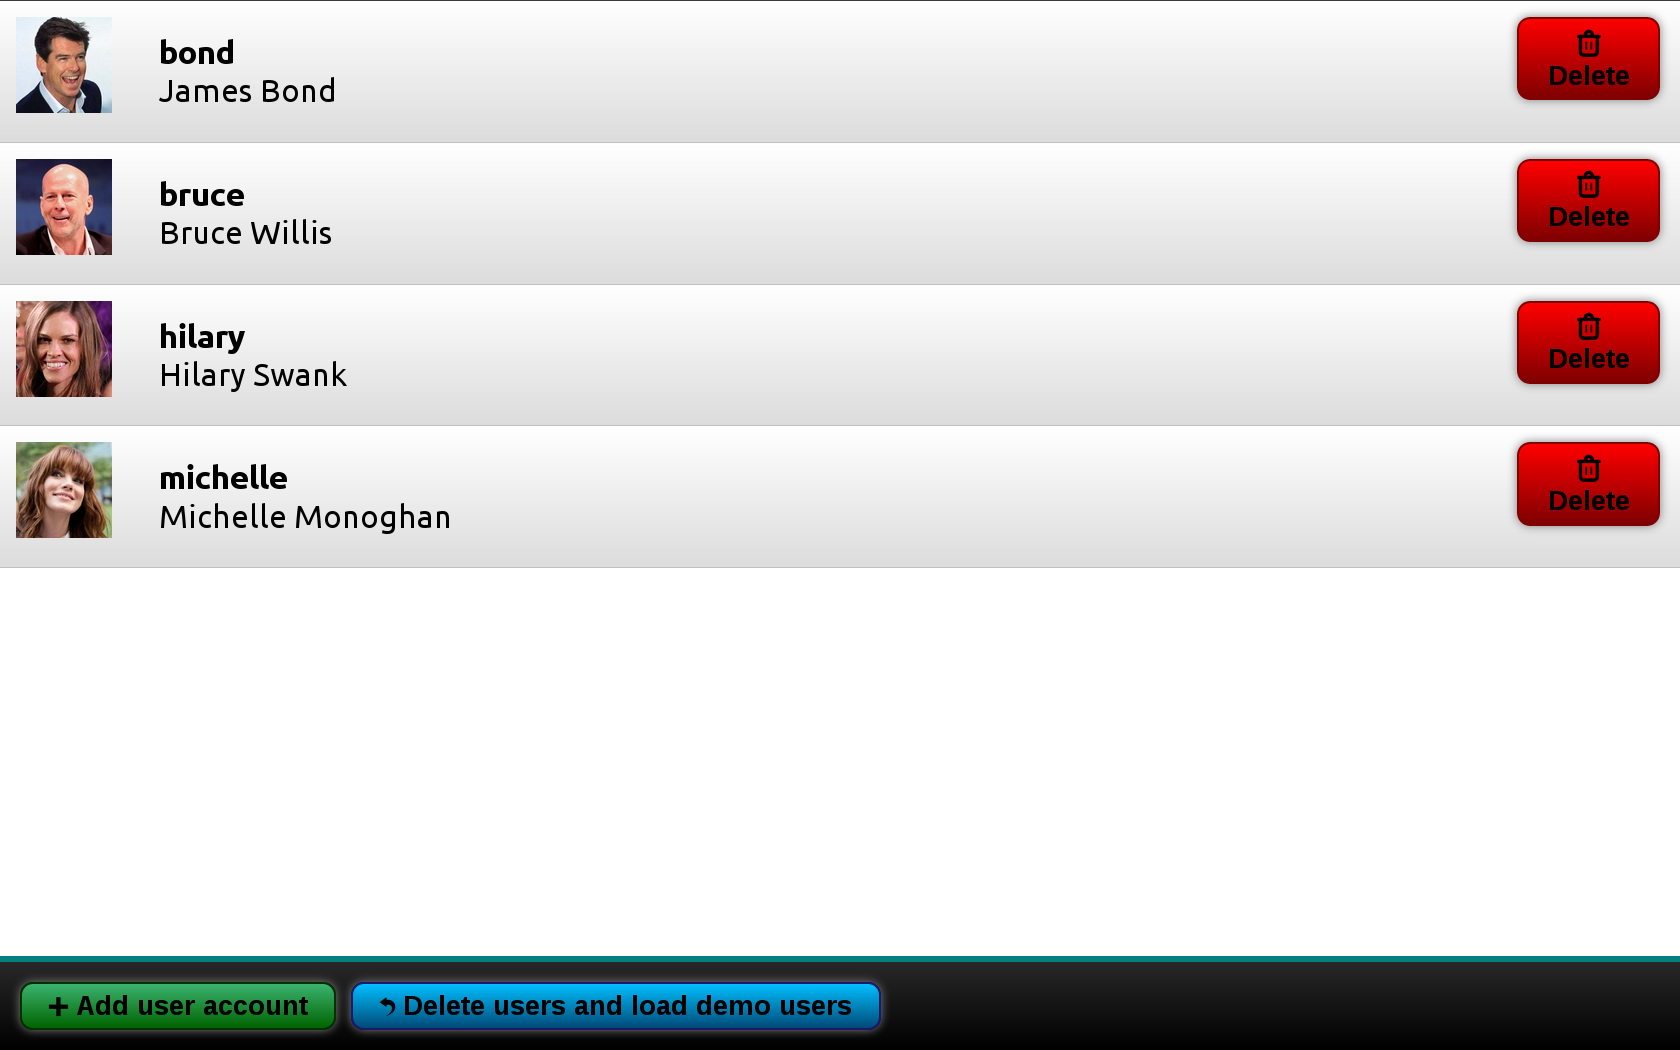
\includegraphics[height=0.325\textheight]{../ui/img/finalUi/accountView.png}
		\caption[Account screen]{Benutzer Verwaltung und Login Screen. Durch klick auf einen Benutzer kann sich der Benutzer mit dessen Konto anmelden.\\
		\license{cc by-sa 3.0 Gage Skidmore, cc by-sa 2.5 Rita Molnár, cc by-sa 3.0 Tabercil, cc by-sa 3.0 Manfred Werner}}
		\label{login screen}
	\end{figure}
	\begin{figure}[H]
		\centering
		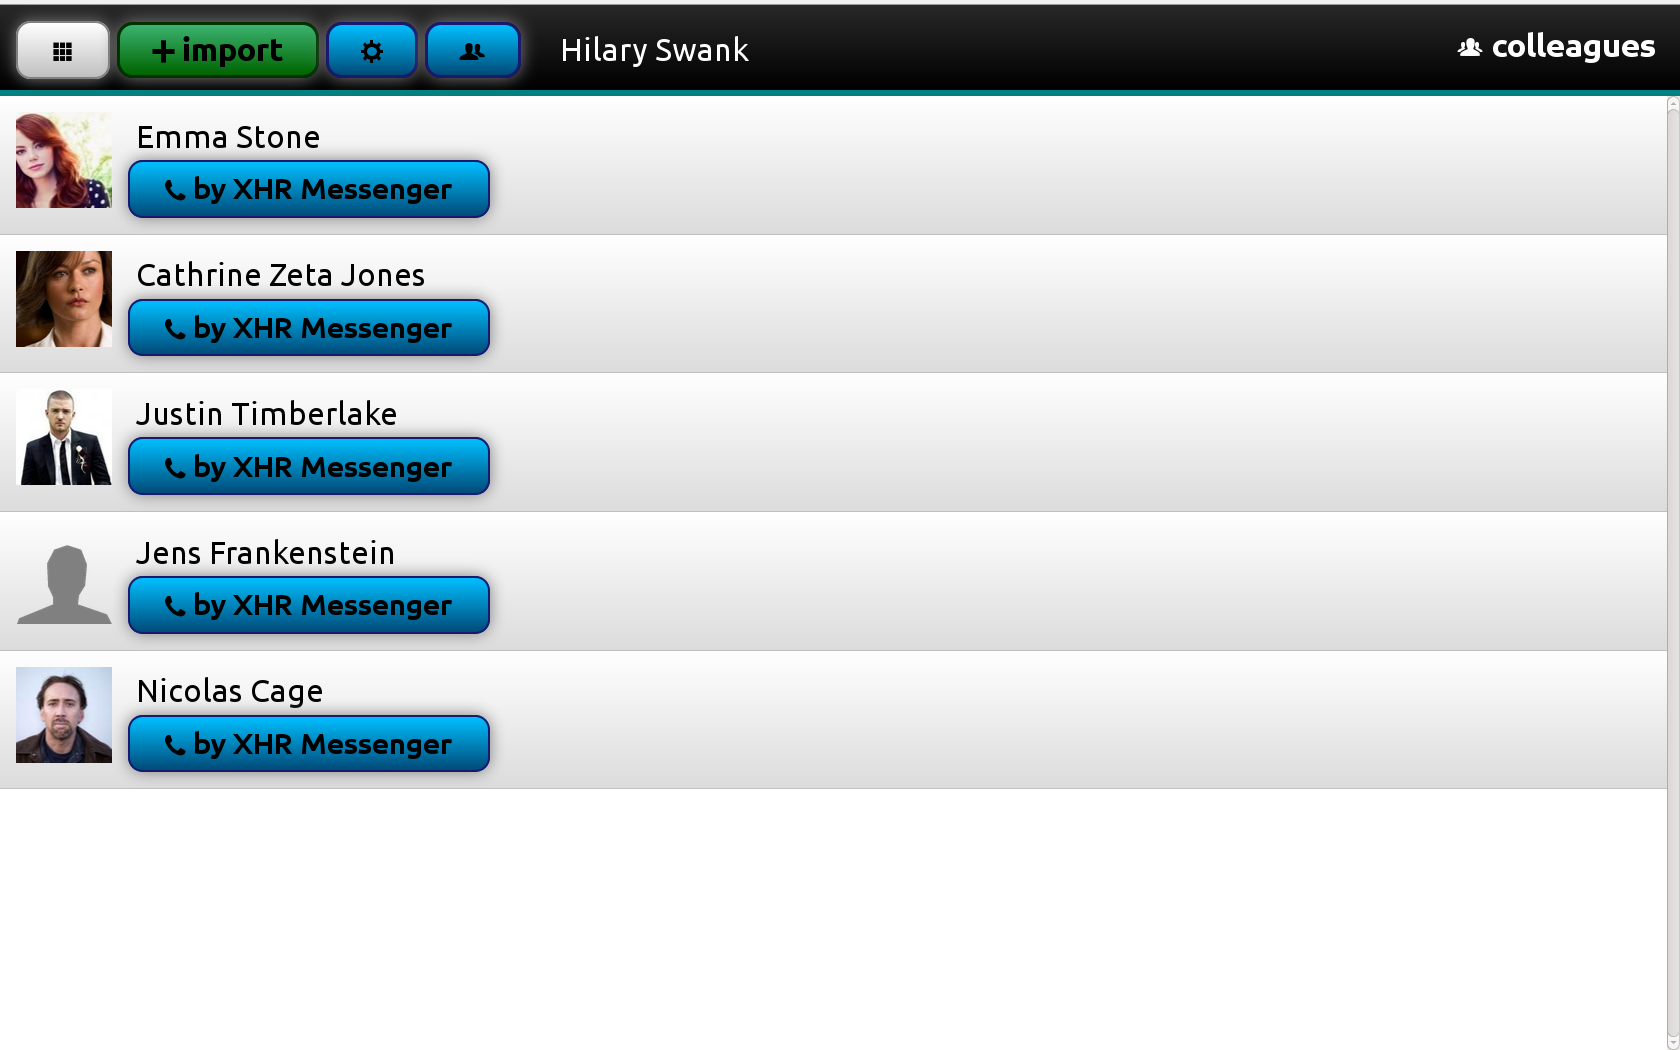
\includegraphics[height=0.325\textheight]{../ui/img/finalUi/contactView1.png}
		\caption[Contactbook screen]{Adressbuch: Von hier aus ruft der Benutzer seine Kontakte an. Die verschiedenen Adressbücher sind über das Listensymbol erreichbar.\\
		\license{cc by-sa 2.0 Gerald Geronimo, cc by 2.0 LeNair Xavier, modified by deerstop, cc by 3.0 Caroline Bonarde Ucci, cc by-sa 2.0 Nicolas Genin}}
		\label{contactbook screen}
	\end{figure}
	\begin{figure}[H]
		\centering
		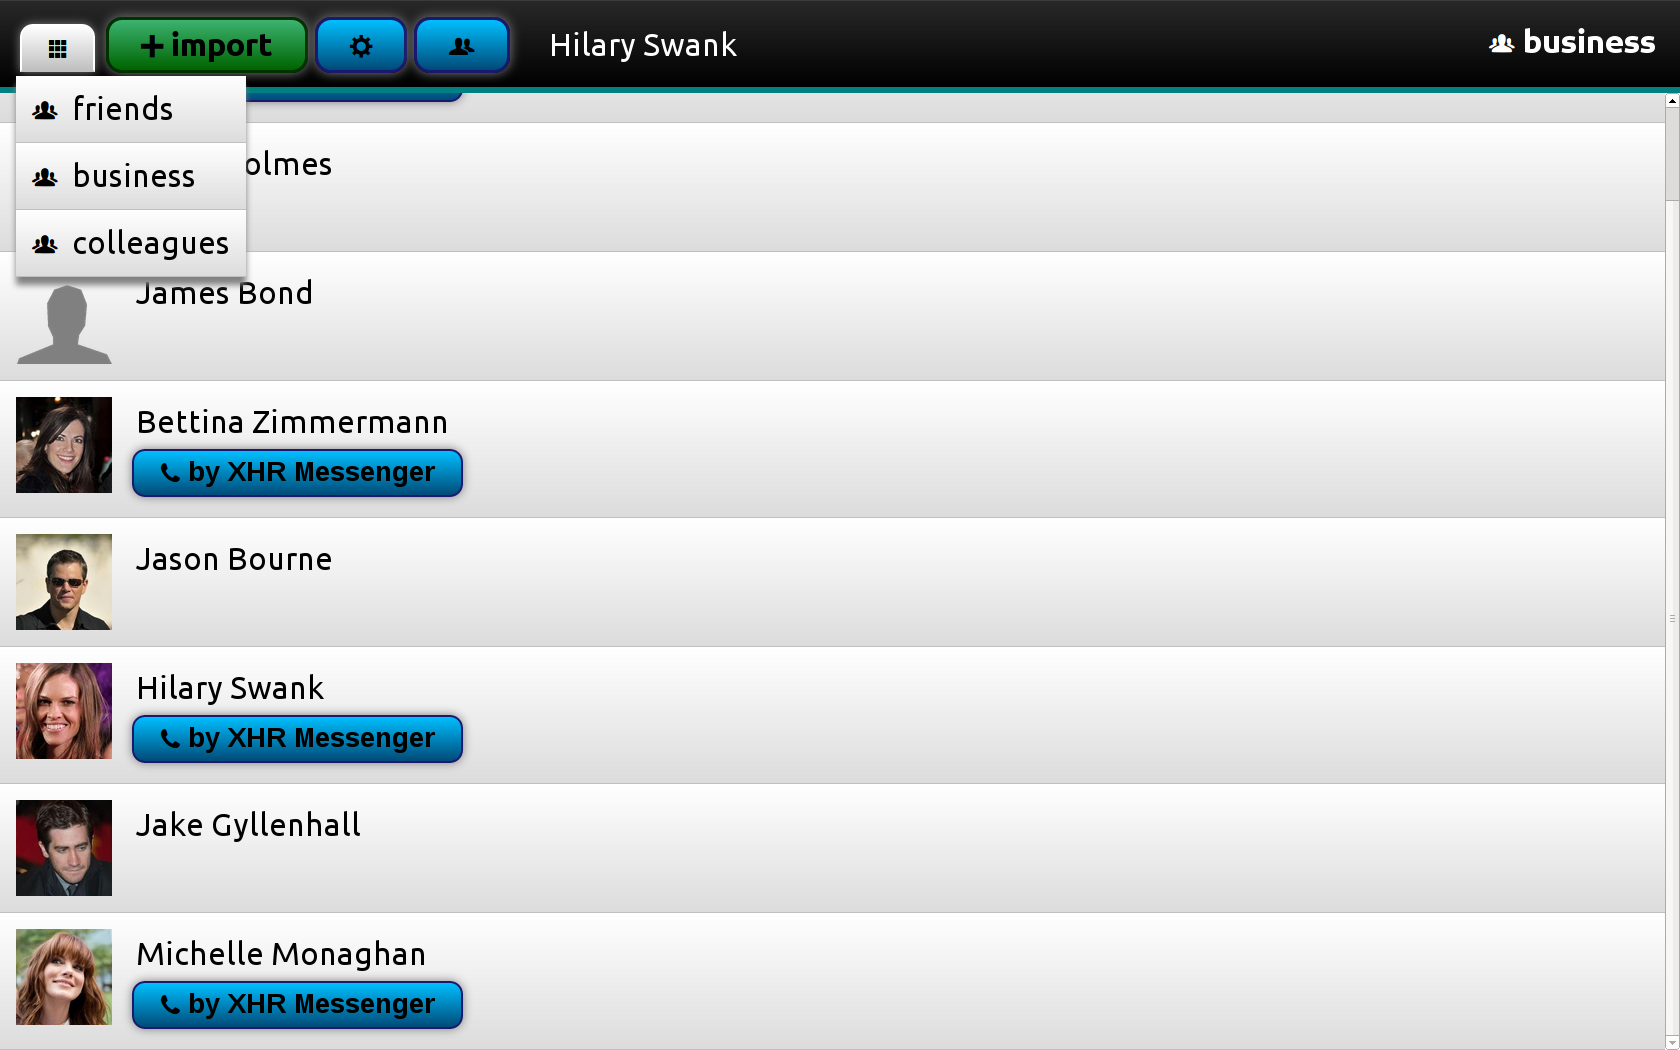
\includegraphics[height=0.4\textheight]{../ui/img/finalUi/contactView2.png}
		\caption[Contactbook list screen]{Auswahl des anzuzeigenden Adressbuches.\\
		\license{cc by 3.0 Siebbi, cc by-sa 2.0 Nicolas Genin, modified by CherryX, cc by-sa 3.0 Manfred Werner, cc by 3.0 Siebbi, cc by-sa 3.0 Tabercil}}
		\label{contactbook change}
	\end{figure}
	\begin{figure}[H]
		\centering
		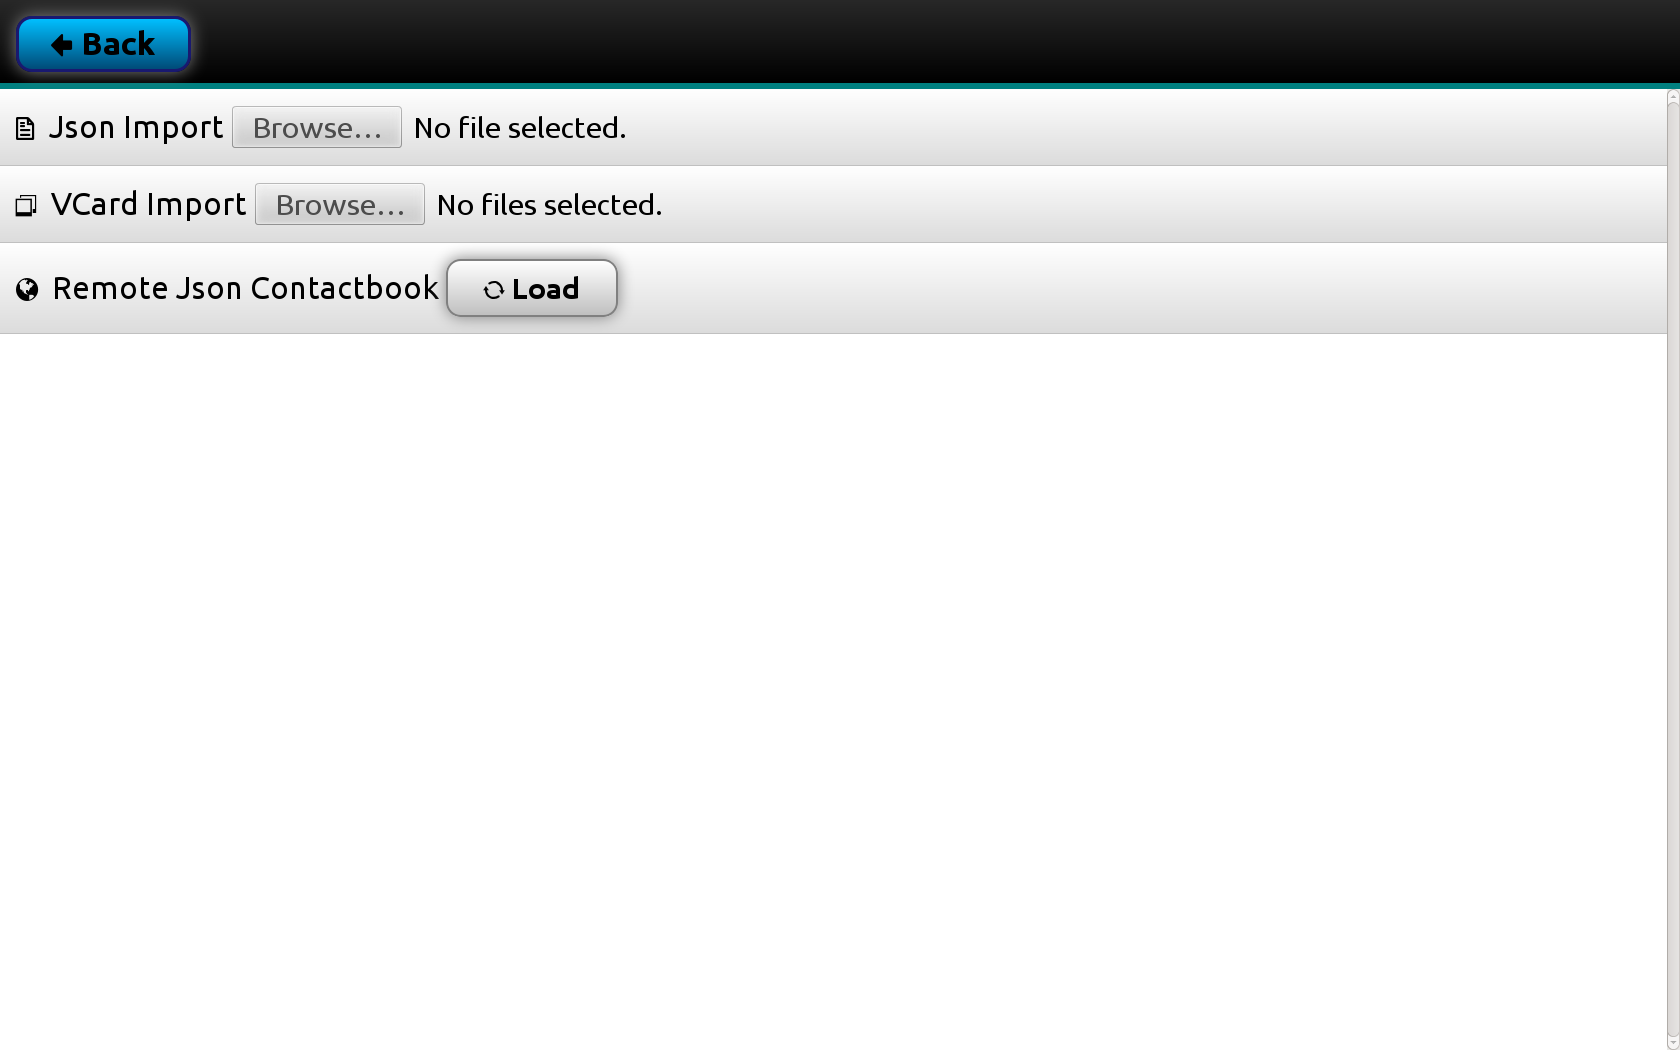
\includegraphics[height=0.4\textheight]{../ui/img/finalUi/importView.png}
		\caption[Contactbook import screen]{Adressbuch Import}
		\label{contactbook import screen}
	\end{figure}
	\begin{figure}[H]
		\centering
		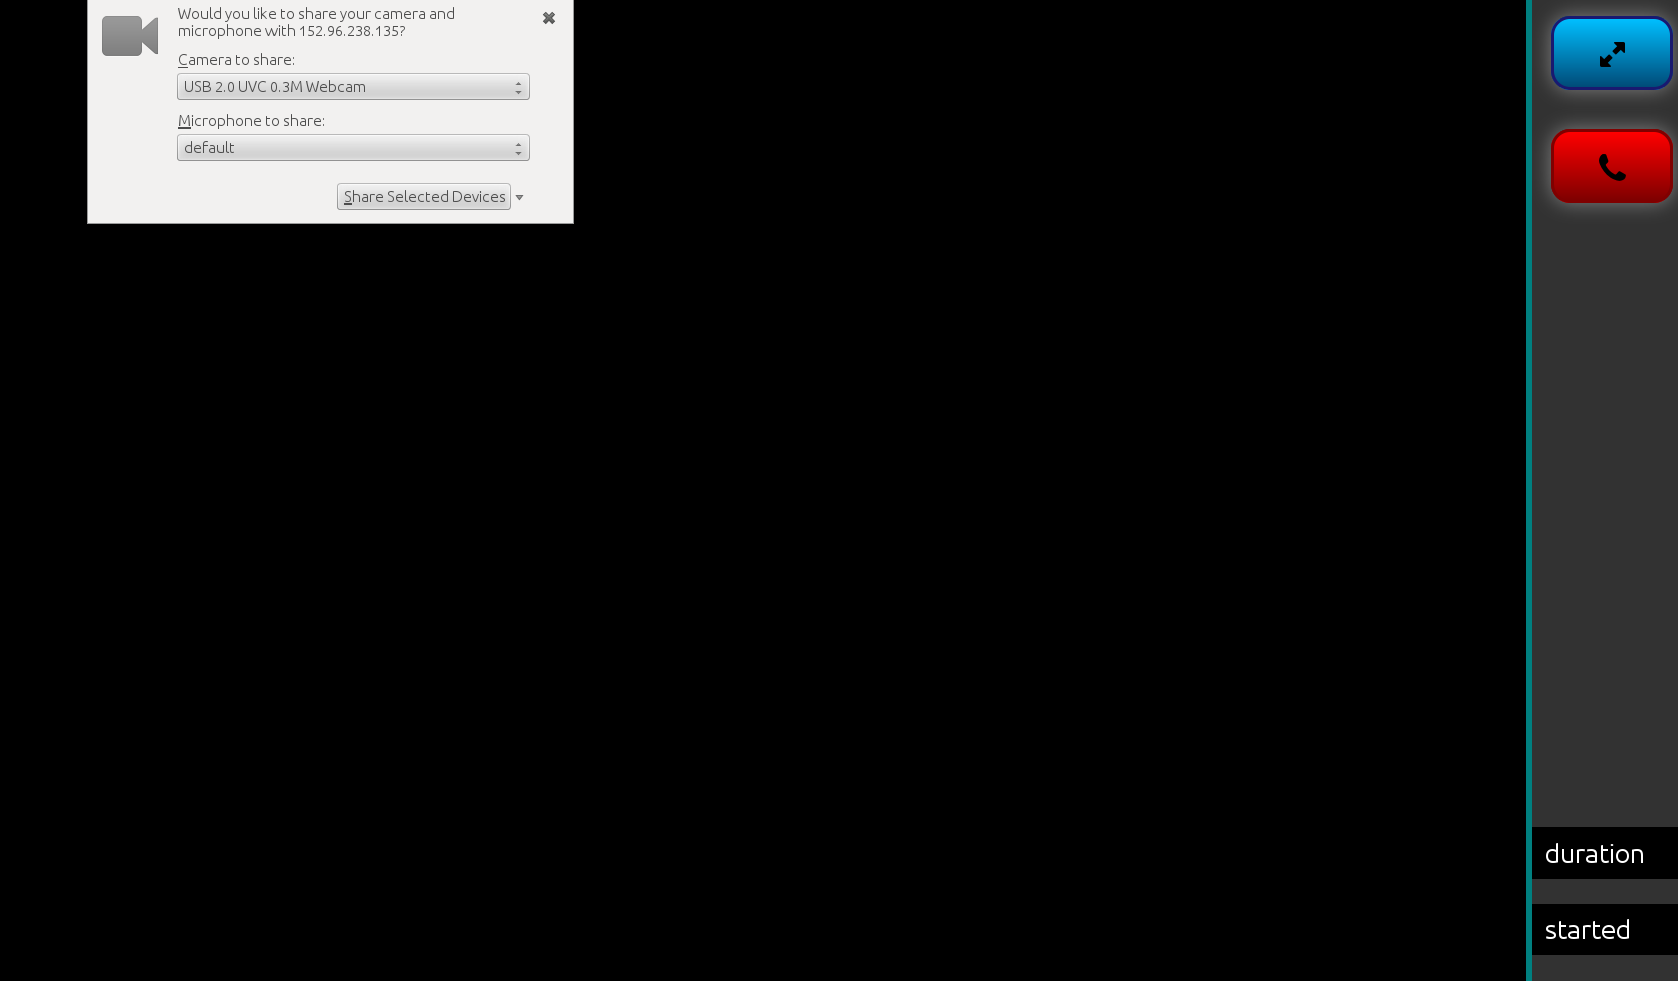
\includegraphics[height=0.4\textheight]{../ui/img/finalUi/cameraAccess.png}
		\caption[Camera access screen]{Anrufen: Kamerazugriff}
		\label{phone screen camera access}
	\end{figure}
	\begin{figure}[H]
		\centering
		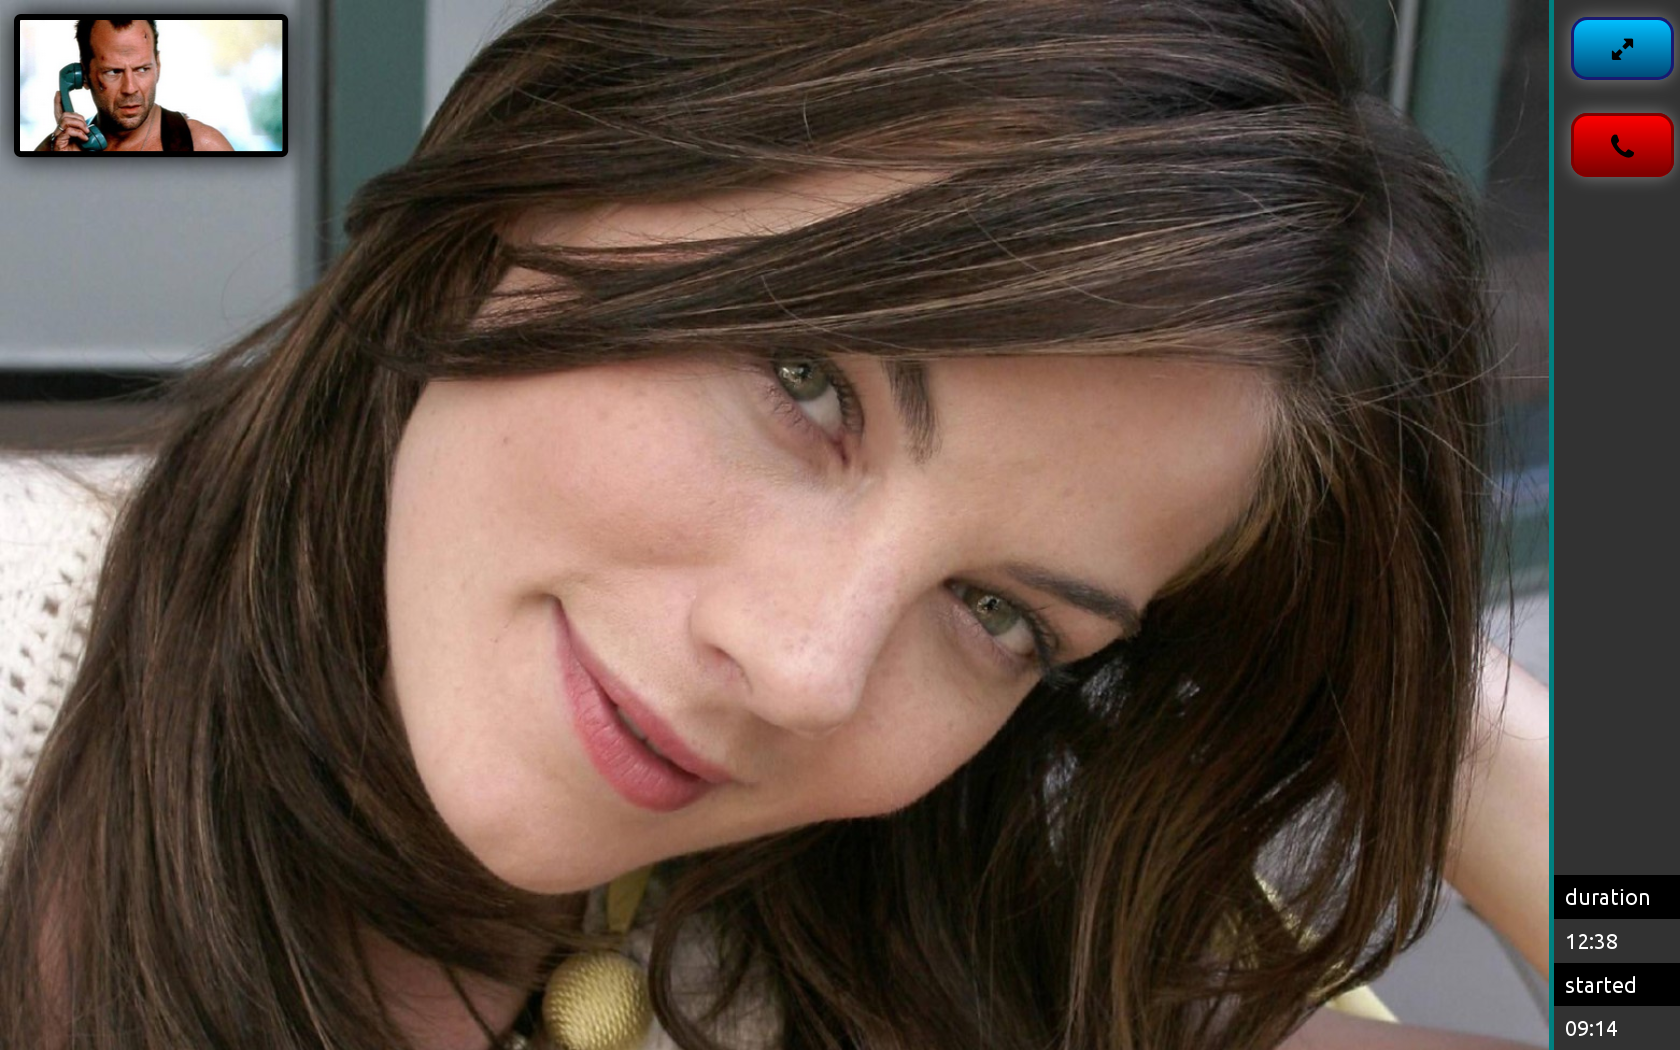
\includegraphics[height=0.4\textheight]{../ui/img/finalUi/phoneView.png}
		\caption[Call screen]{Anrufen}
		\label{phone screen}
	\end{figure}
	\begin{figure}[H]
		\centering
		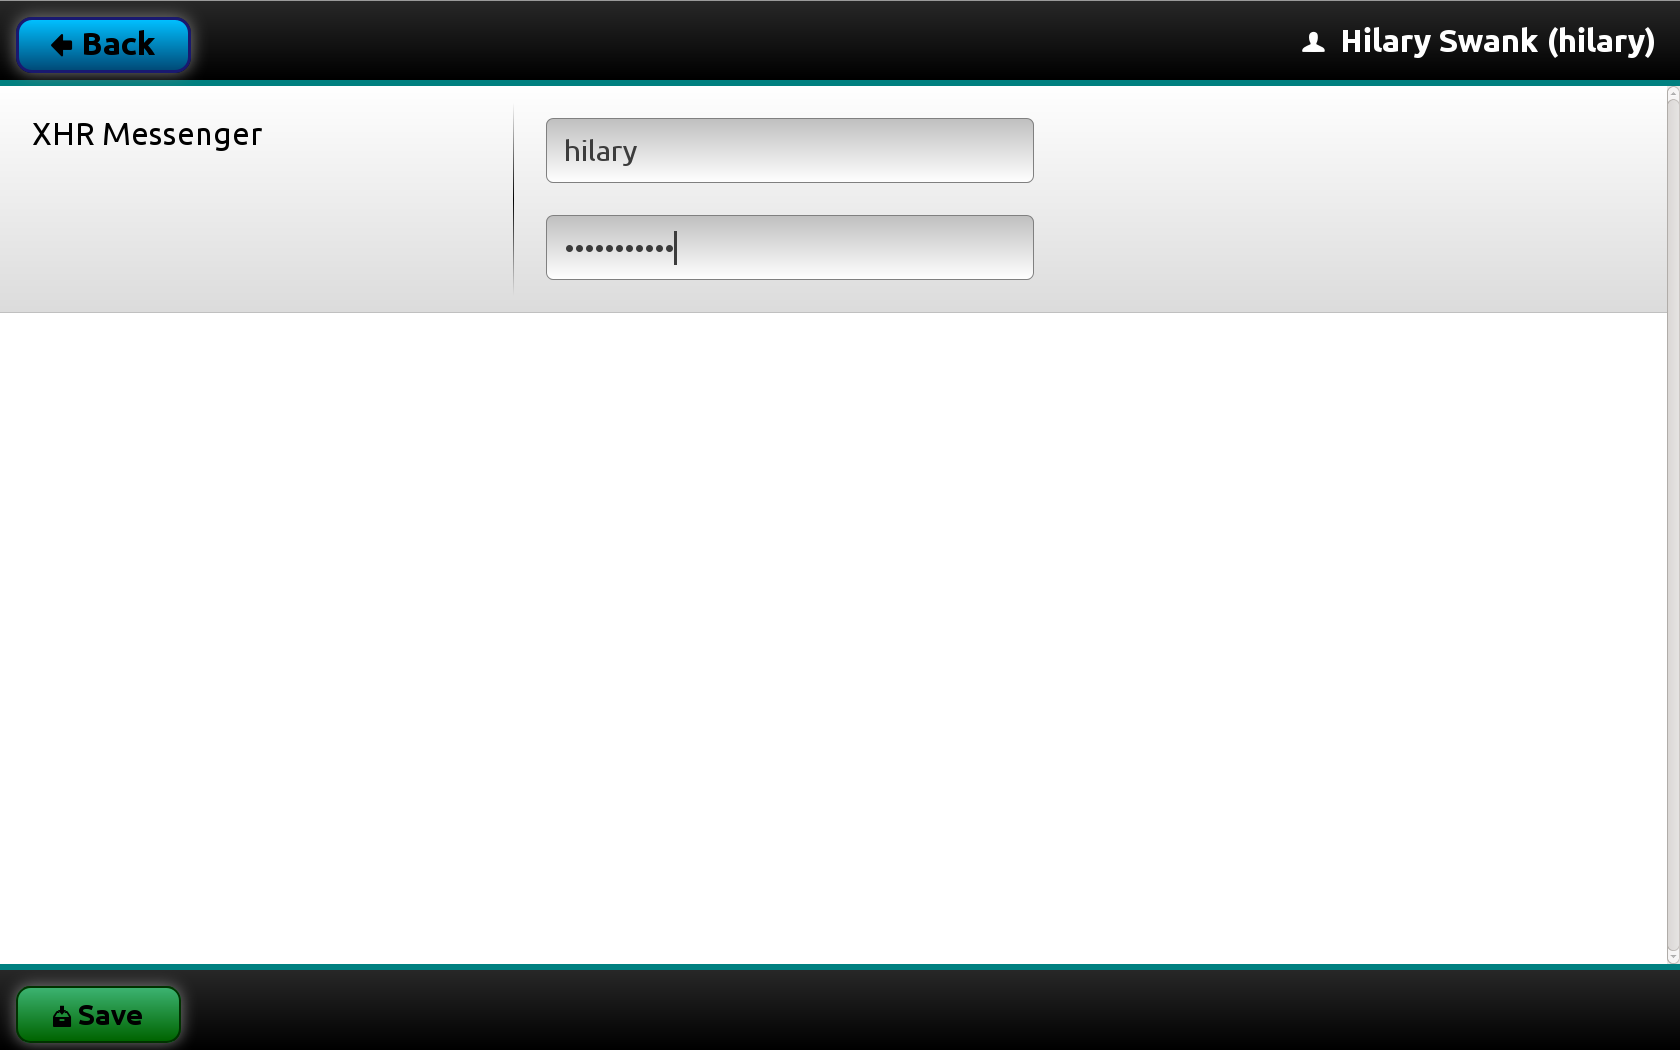
\includegraphics[height=0.4\textheight]{../ui/img/finalUi/accountEditView.png}
		\caption[Channel edit screen]{Account Setting: Verwaltung der Zugänge der aktiven Channels}
		\label{account edit screen}
	\end{figure}

% Performanceanalyse
 \chapter{Performanceanalyse}
	\label{performanceanalyse} 

	
	\begin{landscape}
	\section{Testgeräte}
	\begin{tabularx}{1.4\textwidth}{|l|XXX|}
		\hline
		\textbf{Abbildung} & \textbf{Gerät} & \textbf{Hardware} & \textbf{Software}\\
		\hline
		
\includegraphics[width=3cm]{../performanceAnalaysis/devices/asusux21.png} & Ultrabook, Asus UX 31 & Intel Core i7 2x 1.8 GHz, 3.8GiB Memory
& Ubuntu 12.04 64Bit, Browser: Firefox 25 \\
		\hline
		
\includegraphics[width=3cm]{../performanceAnalaysis/devices/samsungnc10.jpg} & Netbook, Samsung NC 10 & Intel Atom 1.6 GHz, 992MiB Memory & Ubuntu 12.10 32Bit, Browser: Firefox 23 \\
		\hline
		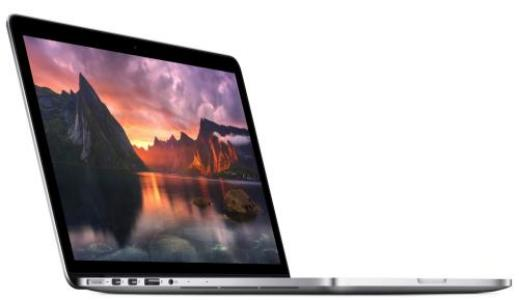
\includegraphics[width=3cm]{../performanceAnalaysis/devices/macbookpro.jpg} & Mac Book Pro 2012 & Intel Core i7 4x 2.3 GHz, 16GB Memory & Mac OS X 10.9 Mavericks, Firefox 24 \\
		\hline
		
\includegraphics[width=3cm]{../performanceAnalaysis/devices/samsunggalaxy101.jpg} & Tablet, Samsung Galaxy Tab 10.1 & Nvidia Tegra 2x 1 GHz, 1GB Memory & Android 4.2.1 32 Bit, Firefox 25 \\
		\hline
		
\includegraphics[width=3cm]{../performanceAnalaysis/devices/googlenexus4.jpg} & Smartphone, Google Nexus 4 & NQualcomm Snapdragon S4 Pro 2x 1.5 GHz, 2GB Memory & Android 4.3 32 Bit, Firefox 25 \\
		\hline
	\end{tabularx}
	
	
	\section{Testszenarien und Ergebnisse}
		Die Tests wurden Bott-Up durchgeführt. Beginnend mit einem Verbindungstest zwischen zwei Browsertabs auf dem gleichen Rechner bis zu einem Test zwischen einem Client im Kabelnetz und einem Client im Mobilfunknetz.
	
		\subsection{Local Round}
			\begin{tabularx}{1.4\textwidth}{|lXX|}
				\hline
				\textbf{Geräte} & \textbf{Setup} & \textbf{Ergebnisse} \\
				\hline
					Ultrabook - Ultrabook
				&
					• 1 Browser\newline 
					• Sender und Empfänger Instanz laufen jeweils in einem Browsertab\newline 
					• Datenverkehr macht roundtripp über Netzwerkkarte\newline 
					• Externe Services wie STUN Service und Signalling Channel
				& 
					• Zunahme CPU Auslastung mit einem Channel: ca 20\%\newline
					• Zunahme Memory Verbrauch: ca 1-2\%\newline
					• Zunahme Netzwerk Trafic: keine da local loop\newline
					• Video Qualität: flüssig, genügend Frames für angenehme Bewegungsdarstellung\newline
					• Die Übertragung wird sauber beendet, keine weitere Leistungsaufnahme sobald der Stream beendet wird.\\
				\hline
			\end{tabularx}
	
			\begin{figure}[H]
				\begin{minipage}[b]{0.5\linewidth}
					\centering
					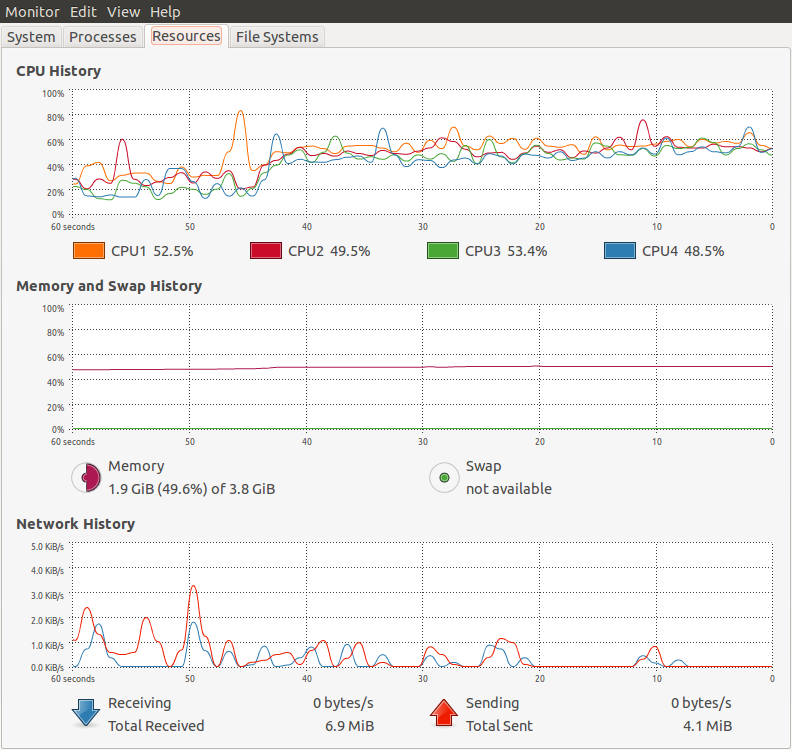
\includegraphics[width=\linewidth]{{../performanceAnalaysis/img/messung1.2.1.1}.png}
					\caption{CPU Leistung für einen Stream}
				\end{minipage}		
				\begin{minipage}[b]{0.5\linewidth}
					\centering
					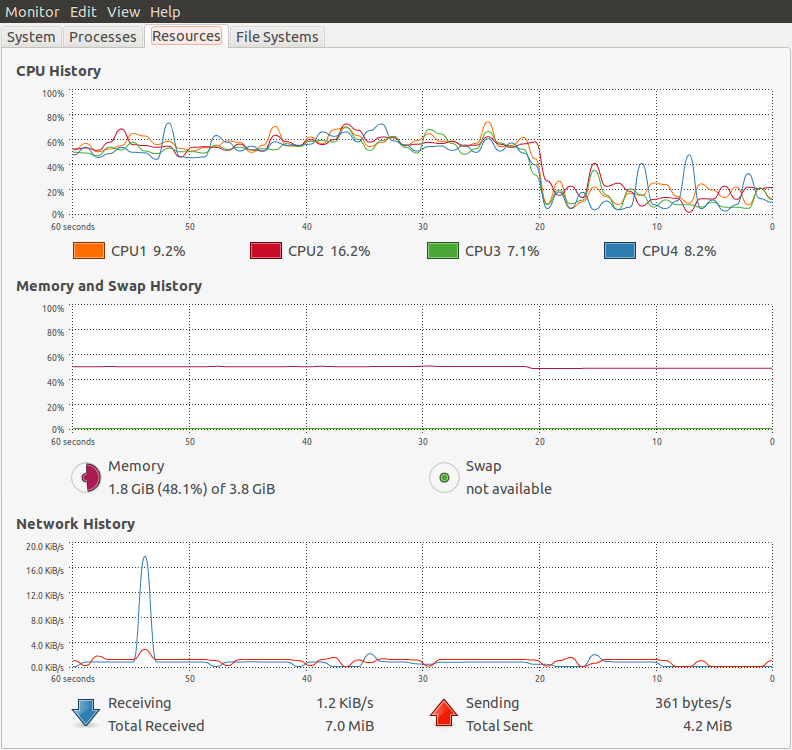
\includegraphics[width=\linewidth]{{../performanceAnalaysis/img/messung1.2.1.2}.png}
					\caption{Vollständige Rückgabe der CPU an andere Prozesse nach dem Ende der Übertragung}
				\end{minipage}
			\end{figure}
			
			
		\subsection{Remote}
			\begin{tabularx}{1.4\textwidth}{|lXX|}
				\hline
				\textbf{Geräte} & \textbf{Setup} & \textbf{Ergebnisse} \\
				\hline
					Ultrabook - Netbook
				&
					• 1 Ultrabook, 1 Netbook\newline 
					• Jeweils gleicher Browser\newline 
					• Datenverkehr läuft über HSR Wlan
				& 
					\textbf{Netbook}:\newline
					• Zunahme CPU Auslastung: ca 50\%\newline
					• Zunahme Memory Verbrauch: nicht spürbar\newline
					• Zunahme Netzwerk Trafic: 10KiB/s out, 15KiB/s\newline
					\textbf{Qualität}: \newline
					• stockend, wenige Frames/s, unbrauchbar für Bewegungsdarstellung\newline
					• Audio Qualität: unbrauchbar\newline
					• Zunahme Netzwerk Trafic: 10KiB/s out, 15KiB/s\\
				\hline				
			\end{tabularx}
			\begin{figure}[H]
				\centering
				\begin{minipage}[b]{0.5\linewidth}
					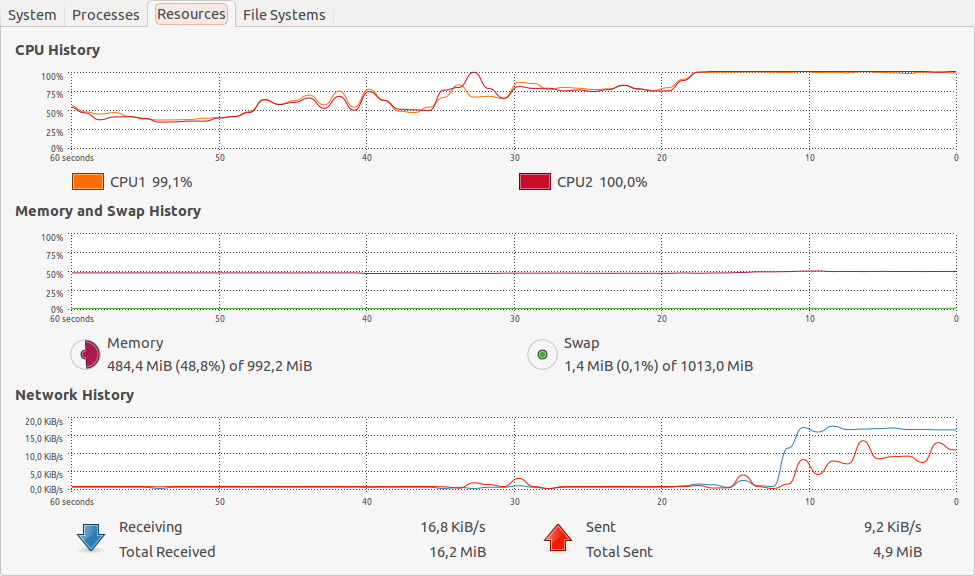
\includegraphics[width=\linewidth]{{../performanceAnalaysis/img/messung2.2.1.1}.png}
					\caption{Das Netbook ist bis an die Leistungsgrenze ausgelastet}
				\end{minipage}
			\end{figure}
			
			
			\begin{tabularx}{1.4\textwidth}{|lXX|}
				\hline
				\textbf{Geräte} & \textbf{Setup} & \textbf{Ergebnisse} \\
				\hline
					Ultrabook - Netbook
				&
					• Gleich wie bei vorherigem Versuch\newline
					• Nur Audio, keine Videoübertragung
				& 
					\textbf{Netbook}:\newline
					• Zunahme CPU Auslastung: ca 20\%\newline
					• Zunahme Memory Verbrauch: nicht spürbar\newline
					• Zunahme Netzwerk Trafic: 7KiB/s in/out\newline
					\textbf{Ultrabook}:\newline
					• Zunahme CPU Auslastung: ca. 10\%\newline
					• Zunahme Memory Verbrauch: nicht spürbar\newline
					• Zunahme Netzwerk Trafic: 8 KiB/s out, 7KiB/s in, Abbruch des Streams nach 30s\\
				\hline				
			\end{tabularx}
			\begin{figure}[H]
				\begin{minipage}[b]{0.5\linewidth}
					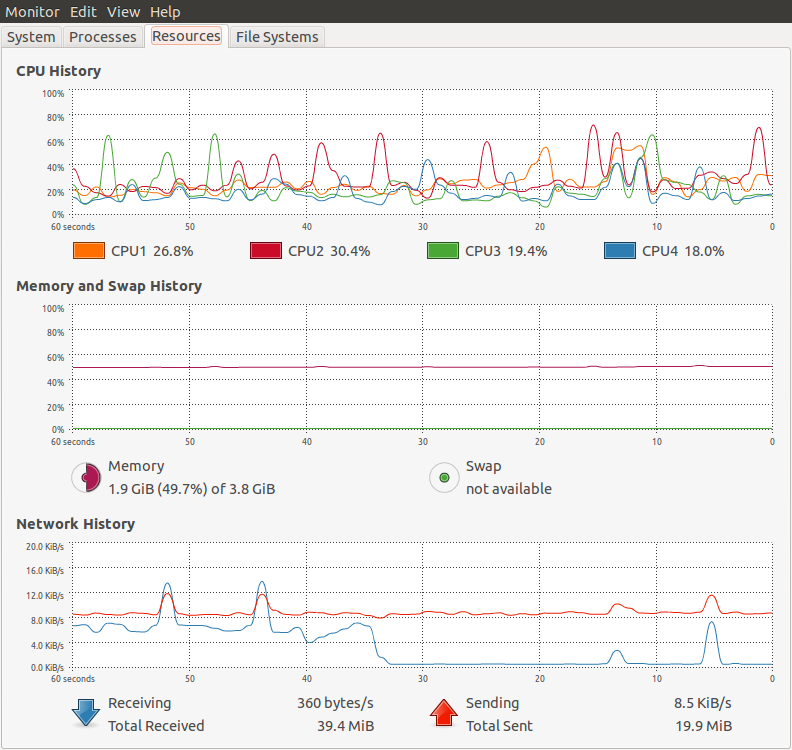
\includegraphics[width=\linewidth]{{../performanceAnalaysis/img/messung2.2.2.1}.png}
					\caption{CPU Belastung Ultrabook}
				\end{minipage}
				\begin{minipage}[b]{0.5\linewidth}
					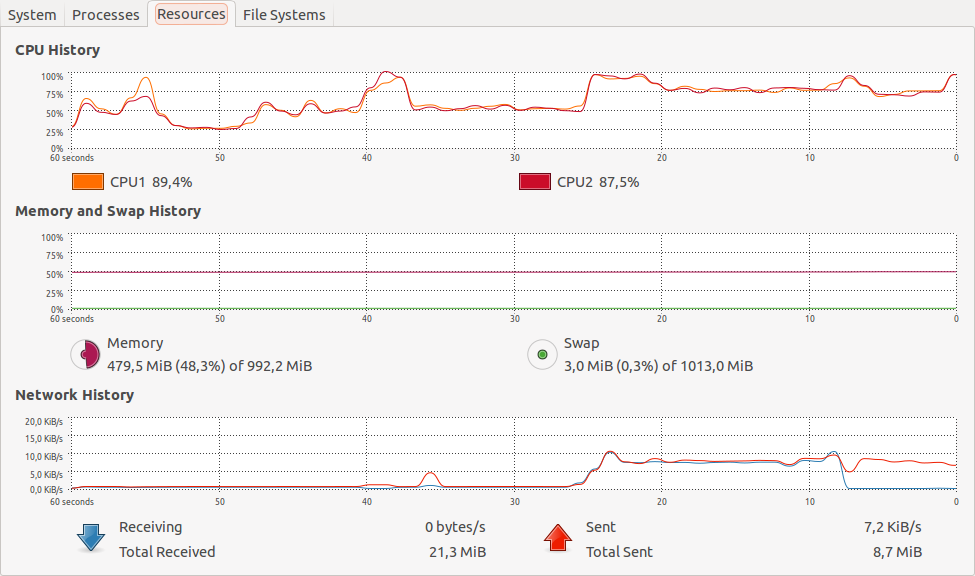
\includegraphics[width=\linewidth]{{../performanceAnalaysis/img/messung2.2.2.2}.png}
					\caption{CPU Belastung Netbook}
				\end{minipage}
			\end{figure}
	
	
			\begin{tabularx}{1.4\textwidth}{|lXX|}
				\hline
				\textbf{Geräte} & \textbf{Setup} & \textbf{Ergebnisse} \\
				\hline
					Ultrabook - Mac Book
				&
					• 1 Ultrabook, 1 Macbook\newline
					• Jeweils gleicher Browser\newline
					• Datenverkehr läuft über HSR Wlan
				& 
					\textbf{Ultrabook}:\newline
					• Zunahme CPU Auslastung: ca 20\%\newline
					• Zunahme Memory Verbrauch: nicht spürbar\newline
					• Zunahme Netzwerk Trafic: 50KiB/s, steigend bis 150KiB/s\newline
					\textbf{Qualität}:\newline
					• Flüssige Audio- und Video Übertragung in beide Richtungen\newline
					• Stream des Macbook's sind keine Einzelbilder sichtbar\newline
					• Stream des Ultrabooks zeigt bei schnellen Bewegungen Einzelbilder\newline
					• Gut geeignet für Bewegungsdarstellung\\
				\hline				
			\end{tabularx}
			\begin{figure}[H]
				\centering
				\begin{minipage}[b]{0.5\linewidth}
					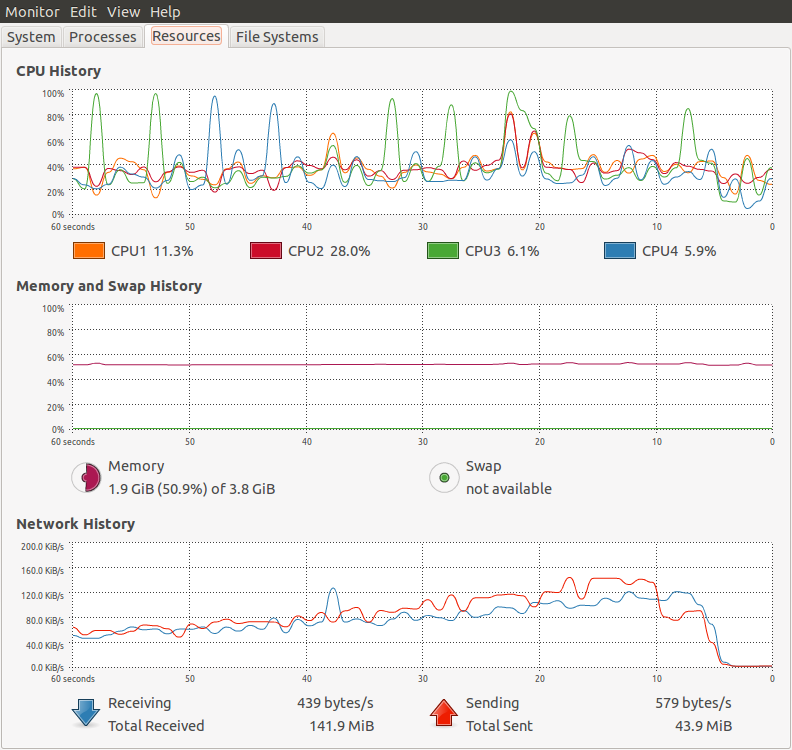
\includegraphics[width=\linewidth]{{../performanceAnalaysis/img/messung2.3.1}.png}
					\caption{Ansteigende (automatisch skalierende) Datenrate, da beide Geräte entsprechende Videoauflösungen liefern können}
				\end{minipage}
			\end{figure}
			
			
		\subsection{Mobile - Desktop}
			\begin{tabularx}{1.4\textwidth}{|lXX|}
				\hline
				\textbf{Geräte} & \textbf{Setup} & \textbf{Ergebnisse} \\
				\hline
					Ultrabook - Tablet
				&
					• 1 Ultrabook, 1 Tablet
					• Beide Geräte im HSR Wlan
				& 
					\textbf{Tablet}:\newline
					• Zunahme CPU Auslastung: ca 70\%\newline
					\textbf{Qualität}:\newline
					• Tablet kann Video vom Desktop flüssig wiedergeben, auch der Ton wird korrekt und verständlich wiedergegeben\newline
					• Tablet bringt Leistung nicht um eigenes Video parallel zum remote zu verarbeiten -> eigenes Video freezed\newline
					• Desktop empfängt entsprechend vom Tablet nur ein Standbild\\
				\hline				
			\end{tabularx}\newline
			
			\noindent
			\begin{tabularx}{1.4\textwidth}{|lXX|}
				\hline
				\textbf{Geräte} & \textbf{Setup} & \textbf{Ergebnisse} \\
				\hline
					Ultrabook - Smartphone
				&
					• 1 Ultrabook, 1 Smartphone
					• Beide Geräte im HSR Wlan
				& 
					\textbf{Qualität}:\newline
					• Video kann sowohl auf dem Phone wie auf dem Desktop einigermassen flüssig wiedergegeben werden\newline
					• Die video Auflösung ist relativ gering\newline
					• Geeignet für Bewegungsdarstellung\\
				\hline				
			\end{tabularx}\newline
			
			\noindent
			\begin{tabularx}{1.4\textwidth}{|lXX|}
				\hline
				\textbf{Geräte} & \textbf{Setup} & \textbf{Ergebnisse} \\
				\hline
					Ultrabook - Smartphone
				&
					• 1 Ultrabook, 1 Smartphone\newline
					• Gleiches Setup wie bei vorherigem Versuch
				& 
					\textbf{Qualität}:\newline
					• Wird das Smartphone gedreht, so verändert die Kamera die Auflösung und refreshed den Stream.\newline
					• Der Stream wird jeweils neu aufgebaut. Dabei wird er auf 40KiB/s gedrosselt und langsam
hochgefahren.\newline
					• Dieses automatische Quality Scaling funktioniert nur, wenn das Gerät dies unterstützt.\newline
					• Das Smartphone wird während der Kommunikation ziemlich warm und warnt bald vor schrumpfender
Akkuleistung.\\
				\hline				
			\end{tabularx}
			\begin{figure}[H]
				\begin{minipage}[b]{0.5\linewidth}
					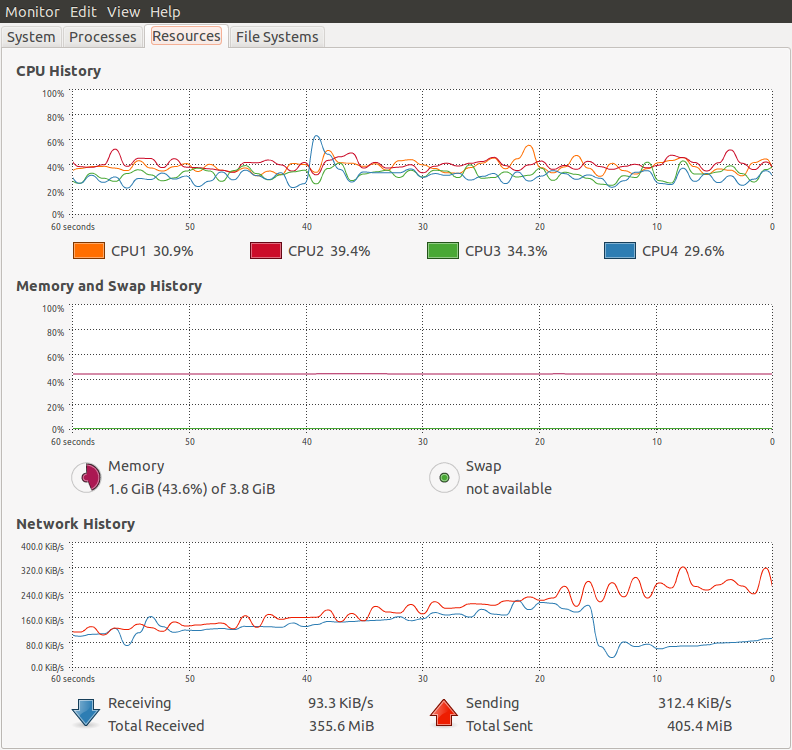
\includegraphics[width=\linewidth]{{../performanceAnalaysis/img/messung3.3.1}.png}
					\caption{Zur Sekunde 25 wird das Smartphone von Widescreen Ausrichtung nach Portrait gedreht. Dabei wird die Datenrate auf das bereits mehrfach beobachtete minimum von 40KiB/s gedrosselt und anschliessend langsam hochgefahren.}
				\end{minipage}
				\begin{minipage}[b]{0.5\linewidth}
					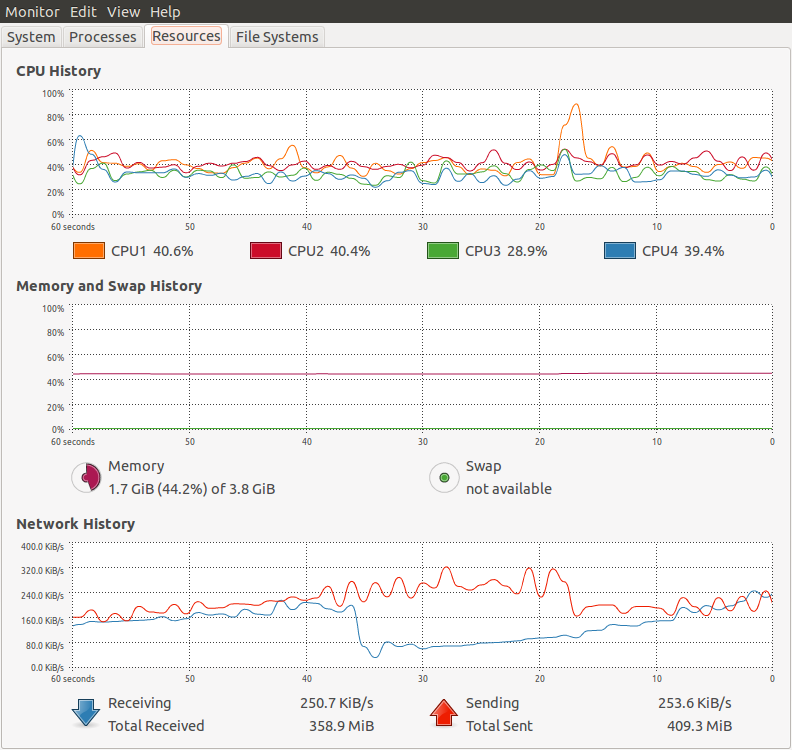
\includegraphics[width=\linewidth]{{../performanceAnalaysis/img/messung3.3.2}.png}
					\caption{Die Datenrate wird bis auf 300KiB/s hochgefahren, wenn die Geräte dies liefern können. Zur 15. Sekunde findet eine Neuausrichtung des Smartphones statt.}
				\end{minipage}
			\end{figure}
			\begin{figure}[H]
				\begin{minipage}[b]{0.5\linewidth}
					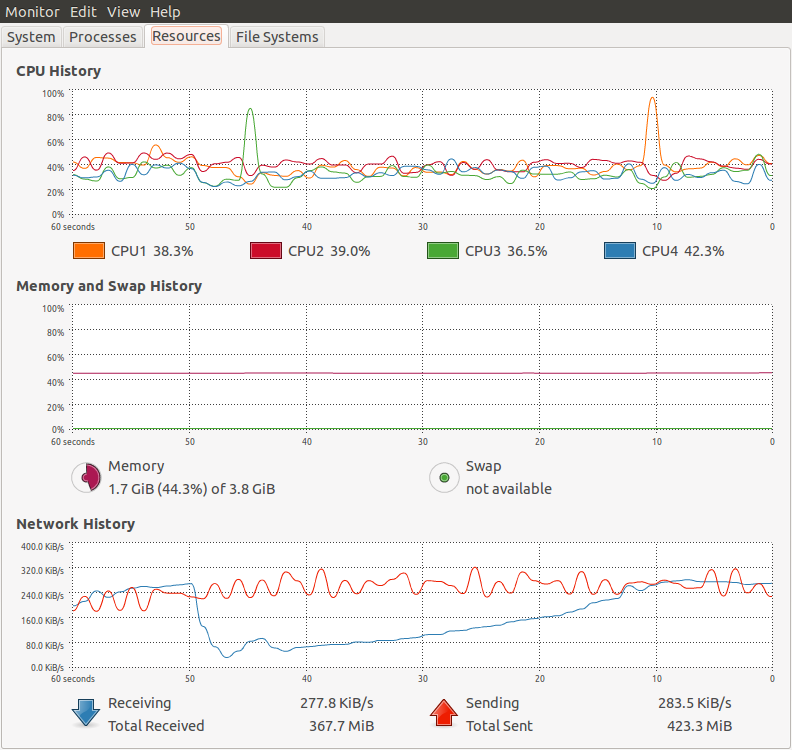
\includegraphics[width=\linewidth]{{../performanceAnalaysis/img/messung3.3.3}.png}
					\caption{Drehung des Smartphone nach Widescreen. Nach 40s erreicht die Auflösung wieder die ursprüngliche Auflösung.}
				\end{minipage}
				\begin{minipage}[b]{0.5\linewidth}
					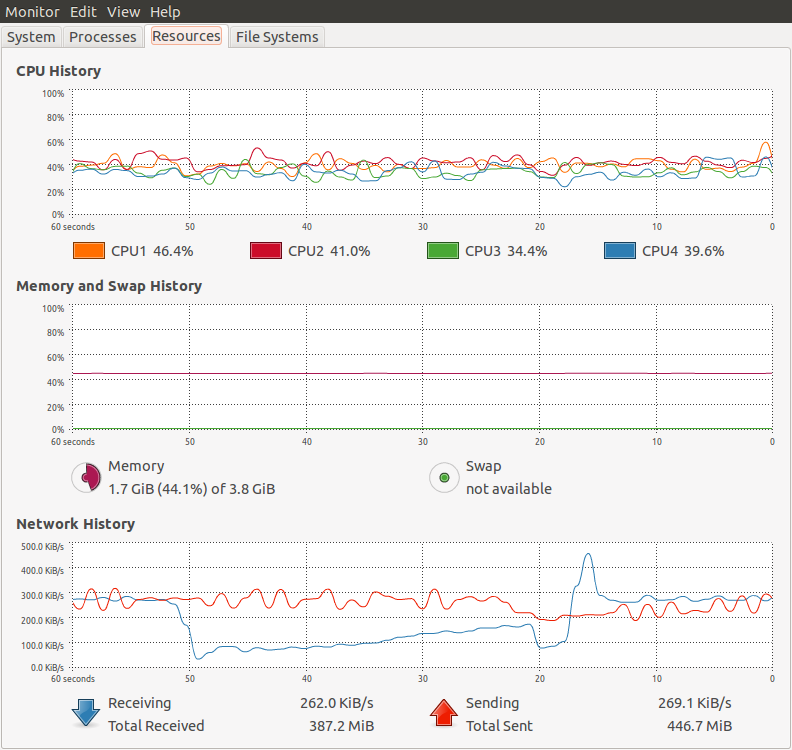
\includegraphics[width=\linewidth]{{../performanceAnalaysis/img/messung3.3.4}.png}
					\caption{Ein Kurzer Pufferunterlauf zur Sekunde 40 führt daraufhin zu einem Peak. Anschliessend pendelt sich die Datenrate bei 300 KiB/s ein.}
				\end{minipage}
			\end{figure}
			
			
		\subsection{Out of Network}
			\begin{tabularx}{1.4\textwidth}{|lXX|}
				\hline
				\textbf{Geräte} & \textbf{Setup} & \textbf{Ergebnisse} \\
				\hline
					Ultrabook - Smartphone
				&
					• 1 Ultrabook, 1 Smartphone\newline
					• Smartphone direkt über Home Wlan angebunden\newline
					• Ultrabook über Home Wlan mit HSR VPN angebunden
				& 
					\textbf{Ultrabook}:\newline
					• Zunahme CPU Auslastung: ca 20\%\newline
					• Zunahme Memory Verbrauch: nicht spürbar\newline
					• Zunahme Netzwerk Trafic: 1-5KiB/s\newline
					• Sprache gut unverständlich\newline
					\textbf{Qualität}:\newline
					• Video stockend oder flüssig, je nach dem ob die Pakete gut durchkommen oder nicht.\newline
					• Smartphone wird etwas warm\newline
					• Video Verzögerung von bis zu ca. 4s\newline
					• Sprache verständlich oder unverständlich, je nach dem wie gut die Übertragungsrate ist.\\
				\hline				
			\end{tabularx}
			\begin{figure}[H]
				\begin{minipage}[b]{0.5\linewidth}
					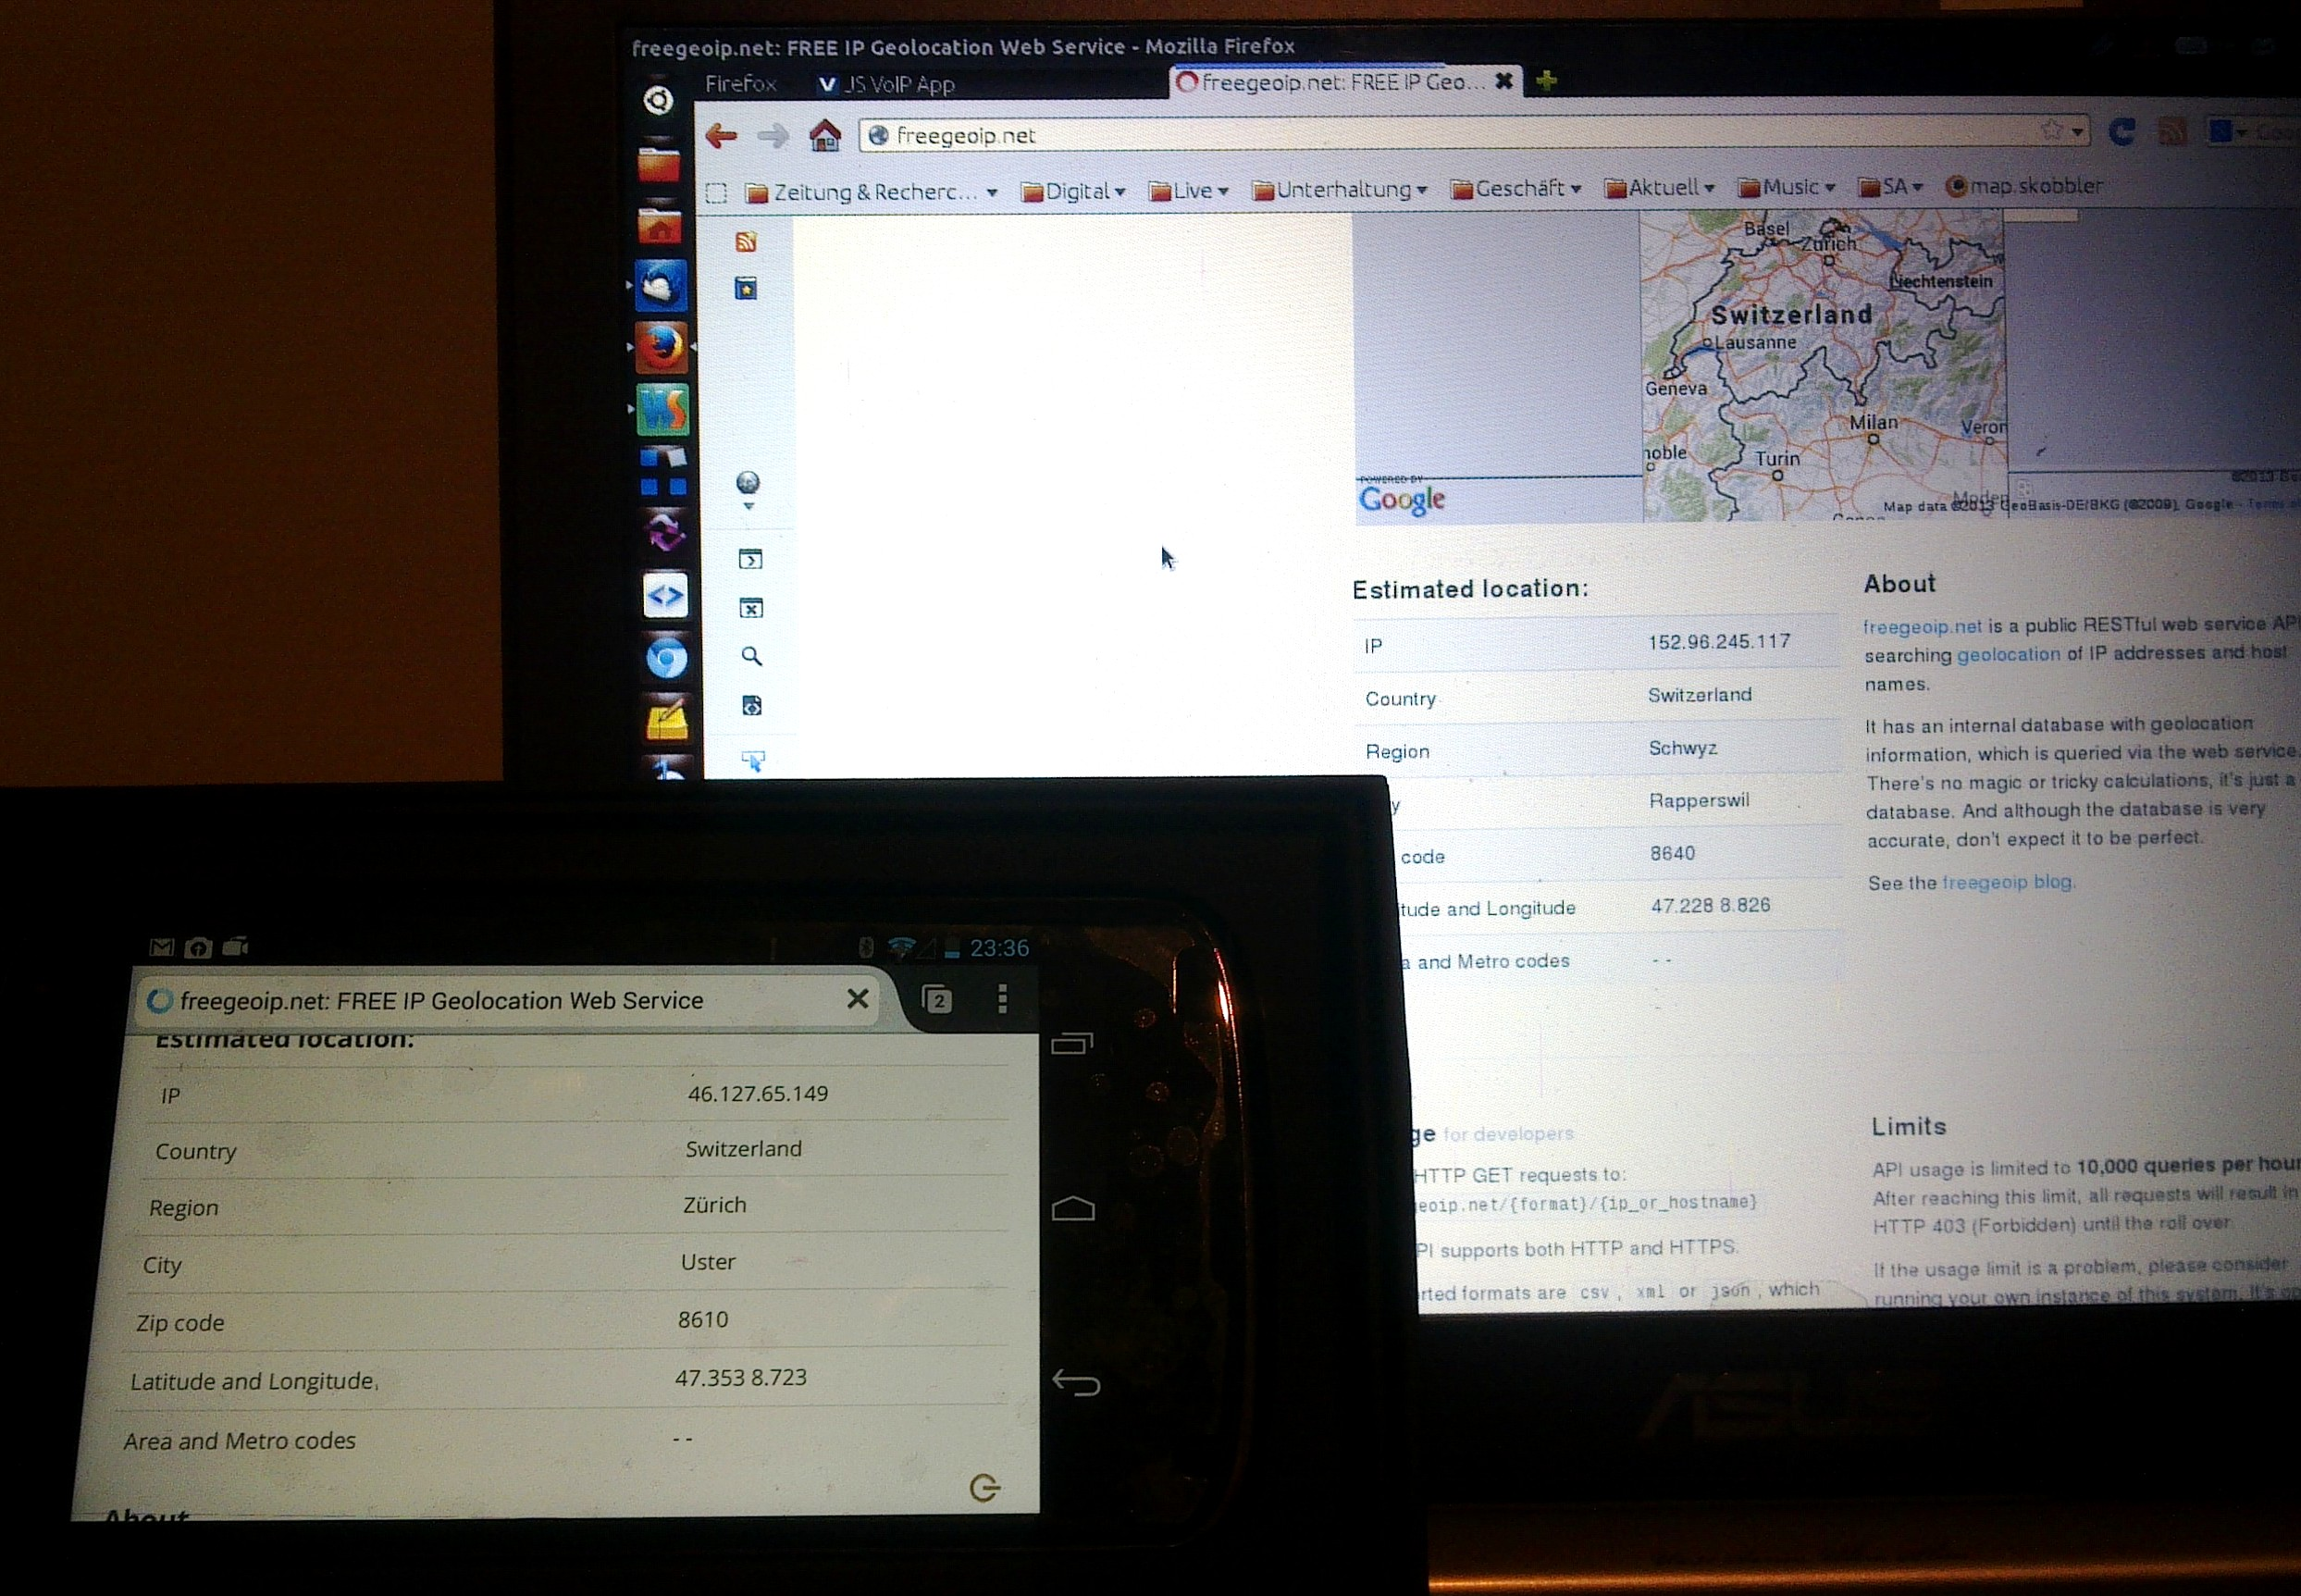
\includegraphics[width=\linewidth]{{../performanceAnalaysis/img/messung4.1setup1}.jpg}
					\caption{freegeoip.net zeigt, das das Ultrabook über die HSR verbunden ist und das Smartphone direkt im lokalen Wlan hängt.}
				\end{minipage}
				\begin{minipage}[b]{0.5\linewidth}
					\includegraphics[width=\linewidth]{{../performanceAnalaysis/img/messung4.1.1}.png}
					\caption{Das Ultrabook kann einige wenige KiB/s liefern, das Smartphone sogar nut 1KiB/s.}
				\end{minipage}
			\end{figure}			
			\begin{figure}[H]
				\begin{minipage}[b]{0.5\linewidth}
					\includegraphics[width=\linewidth]{{../performanceAnalaysis/img/messung4.1.3.1}.jpg}
					\caption{Videokommunikation zwischen Smartphone und Ultrabook}
				\end{minipage}
				\begin{minipage}[b]{0.5\linewidth}
					\includegraphics[width=\linewidth]{{../performanceAnalaysis/img/messung4.1.2}.png}
					\caption{Die Datenrate fährt hoch bis über 100 KiB/s. Drehung des Smartphones zur Sekunde 55}
				\end{minipage}
			\end{figure}
			
		\subsection{Festnetz - Mobilfunknetz}
			\begin{tabularx}{1.4\textwidth}{|lXX|}
				\hline
				\textbf{Geräte} & \textbf{Setup} & \textbf{Ergebnisse} \\
				\hline
					Ultrabook - Netbook
				&
					• 1 Ultrabook, 1 Netbook\newline
					• Netbook über UMTS (Stadt) angebunden\newline
					• Ultrabook über Home Wlan angebunden\newline
					• 1. Mal Video+Audio, 2. Mal nur Audio
				& 	
					\textbf{Ultrabook}:\newline
					• Zunahme Netzwerk Trafic bei Video: ca32-70KiB/s\newline
					• Zunahme Netzwerk Trafic bei Audio: ca8KiB/s\newline
					\textbf{Qualität (Video)}:\newline
					• Video stockend\newline
					• Audio verzögert und nur knapp verständlich\newline
					\textbf{Qualität (nur Audio)}:\newline
					• Audio flüssig, kaum verzögert und gut verständlich\\
				\hline	
			\end{tabularx}
			\begin{figure}[H]
				\begin{minipage}[b]{0.5\linewidth}
					\includegraphics[width=\linewidth]{{../performanceAnalaysis/img/messung5.1.1}.png}
					\caption{Ultrabook: Die Videowiedergabe ist nach dem Start noch relativ schmalbandig}
				\end{minipage}
				\begin{minipage}[b]{0.5\linewidth}
					\includegraphics[width=\linewidth]{{../performanceAnalaysis/img/messung5.1.2}.png}
					\caption{Netbook: Die Datenrate vom Ultrabook ist etwas höher als die des Netbook.}
				\end{minipage}
			\end{figure}			
			\begin{figure}[H]
				\begin{minipage}[b]{0.5\linewidth}
					\includegraphics[width=\linewidth]{{../performanceAnalaysis/img/messung5.1.3}.png}
					\caption{Ultrabook: Audiodatenrate nach dem Verbinden}
				\end{minipage}
				\begin{minipage}[b]{0.5\linewidth}
					\includegraphics[width=\linewidth]{{../performanceAnalaysis/img/messung5.1.4}.png}
					\caption{Netbook: Audiodatenrate nach einiger Zeit (eingependelt)}
				\end{minipage}
			\end{figure}	
	
	\end{landscape}
	
	

% Firewall Testing
\begin{landscape}

\chapter{Firewall Testing}
	\label{firewalltesting}

	
	\section{Testgeräte}
	\begin{tabularx}{1.4\textwidth}{|l|XXX|}
		\hline
		\textbf{Abbildung} & \textbf{Gerät} & \textbf{Hardware} & \textbf{Software}\\
		\hline
		\includegraphics[width=3cm]{../performanceAnalaysis/devices/asusux21.png} & Ultrabook, Asus UX 31 & Intel Core i7 2x 1.8 GHz, 3.8GiB Memory
& Ubuntu 12.04 64Bit, Browser: Firefox 25 \\
		\hline
		\includegraphics[width=3cm]{../performanceAnalaysis/devices/samsungnc10.jpg} & Netbook, Samsung NC 10 & Intel Atom 1.6 GHz, 992MiB Memory & Ubuntu 12.10 32Bit, Browser: Firefox 23 \\
		\hline
		\includegraphics[width=3cm]{../performanceAnalaysis/devices/googlenexus4.jpg} & Smartphone, Google Nexus 4 & NQualcomm Snapdragon S4 Pro 2x 1.5 GHz, 2GB Memory & Android 4.3 32 Bit, Firefox 25 \\
		\hline
	\end{tabularx}
	
	
	\section{Testszenarien und Ergebnisse}
	
		\subsection{VPN - Home-WLAN}
			\begin{tabularx}{1.4\textwidth}{|lXX|}
				\hline
				\textbf{Geräte} & \textbf{Setup} & \textbf{Ergebnisse} \\
				\hline
					Home-WLAN - Home-WLAN-HSR-VPN
				&
					• Smartphone über Home-WLAN, Cablecom 10er-Leitung\newline
					• Ultrabook über Home-WLAN, Cablecom 10er-Leitung,
					Verbunden mit HSR-VPN\newline
				& 
					• Media-Stream kommt ohne Verzögerung zustande\newline
					• Kein Unterschied zu Locale Round\\
				\hline
			\end{tabularx}
			
			
		\begin{figure}[H]
			\centering
			\begin{minipage}[b]{0.5\linewidth}
				\includegraphics[width=\linewidth]{{../performanceAnalaysis/img/messung4.1setup1}.jpg}
				\caption{freegeoip.net zeigt, das das Ultrabook über die HSR verbunden ist und das Smartphone direkt im lokalen Wlan hängt.}
			\end{minipage}
		\end{figure}
	
		\subsection{HSR - Mobile}
			\begin{tabularx}{1.4\textwidth}{|lXX|}
				\hline
				\textbf{Geräte} & \textbf{Setup} & \textbf{Ergebnisse} \\
				\hline
					Mobile Network - HSR-Notebook-WLAN
				&
					• Netbook über Mobilfunk, Sunrise Mobile Prepaid (max. 256 Kbps)\newline
					• Ultrabook über HSR-Notebook-WLAN\newline
				& 
					• Media-Stream kommt nicht zustande\newline
					• Im Wireshark sind keine UDP-Pakete sichtbar\newline
					• Vermutung: HSR blockt ``dynamic port"'-``dynamic port"'-Verbindungen um
					Filesharing zu unterbinden\newline
					• Auch die apprtc.appspot.com-Demo-App kommt nicht durch\\
				\hline
			\end{tabularx}
			
		\subsection{Home-WLAN - Mobile}
			\begin{tabularx}{1.4\textwidth}{|lXX|}
				\hline
				\textbf{Geräte} & \textbf{Setup} & \textbf{Ergebnisse} \\
				\hline
					Mobile Network - Home-WLAN
				&
					• Netbook über UMTS (Stadt)\newline
					• Ultrabook über Home-WLAN
				& 	
					• Media-Stream wird erfolgreich aufgebaut\\
				\hline	
			\end{tabularx}
				
\end{landscape}


% Qualitätsmanagement
\chapter{Qualitätsmanagement}
	Zur Sicherung der Qualität wurden verschiedene Strategien kombiniert. Zur automatisierten Qualitätskontrolle wurden Unittests eingesetzt. Die Performance und das Verbindungsverhalten durch Firewalls hindurch wurde durch systematische Tests ermittelt. Die Funktion der Benutzeroberfläche wurde durch regelmässige manuelle Tests in Firefox und Chrome überprüft.
	Die Connection und die Videokommunikation wurden durch regelmässige manuelle Tests zu zweit mit zwei Geräten getestet.
	
	\begin{figure}[H]
		\centering
		{\tiny
			\csvautotabular{../qualityManagement/timelog.csv}
		}
		\caption{Die Aktivität "`Qualitätsmanagement"' fasst Testing und Reviewing
		zusammen.}
	\end{figure}

	\section{Automatisierte Tests}
		\begin{description}
			\item[Unittests]		
			\begin{figure}[H]
				\centering
				\includegraphics[width=1\textwidth]{../qualityManagement/unittesting.png}
				\caption{mit QUnit erfolgreich ausgeführte Tests}
				\label{unittests}
			\end{figure}
			Die Applikationsdomain wird mit Unittests getestet und die fortbleibende
			Funktion bei Änderungen damit nachgewiesen.
		\end{description}
		
	\section{Systematische Tests}
		\begin{description}
			\item[Performancetest]
			Die Performance wurde durch eine umfangreiche Performanceanalyse untersucht und dokumentiert. Dabei wurden Mobilgeräte wie Desktopgeräte getestet.
		
			Siehe Anhang \ref{performanceanalyse}
		
			\item[Firewall Tests]
			Das Verhalten der durch WebRTC genutzten Protokolle durch Firewalls hindurch wurde in einem dreiteiligen Firewall-Test ermittelt. Dabei wurde das Verhalten der HSR Firewall, von Firewalls in Mobilfunk- und von Firewalls in Heimnetzanbindungen untersucht. 
		
			Siehe Anhang \ref{firewalltests}
		\end{description}
		
	\section{Manuelle Tests}
		\begin{description}
			\item[Connection \& Videoverbindung]
			Die Connection stellt die am schwierigsten zu testende Komponente und gleichfalls eine der komplexeren dar, weil sie die RTCPeerConnection, die RTCDataChannel und die UserMedia Schnittstelle verwendet. Die Schnittstellen interagieren mit dem User und mit Netzwerkevents. Testen mit Unittests wäre nur möglich gewesen, wenn für diese Schnittstellen komplette Dummies gebaut worden wären. 
		
			Aus diesem Grund wurde als Teststrategie manuelles Testen gewählt. Dabei wurden Verbindungsaufbau und -abbau jeweils in jeder Richtung mit Firefox, Chrome und Firefox-Chrome kombiniert sowie allen Variationen von Auf- und Abbaureihenfolgen zu zweit mit zwei Geräten durchgetestet.
	
			Dies wurde in jeder Iteration mindestens einmal durchgeführt um die Funktionalität zu überprüfen.
		
			\item[Kontaktbuch Import] Die Verarbeitung der Kontaktbuchdaten und das Kontaktbuchmanagement haben wir durch Unittests abgedeckt.
			Beim Import hätten wir ebenfalls einen Dummy bauen müssen. Daher wurde auch diese manuel getestet.
		\end{description}
			
		
	\section{Reviews}
		Regelmässige Reviews stellten die Qualität von Dokumentation und Code sicher. Für die Reviews wurde die Commit-Kommentarfunktion von GitHub genutzt.
		
		Zusätzlich hat uns Herr Bläser ein Code Review durchgeführt.


% interfaces & protocols
\chapter{Schnittstellen \& Protokolle}
	\begin{description}
		\item[Channel] Beschreibt die Channelschnittstelle. Implementatoren eines eigenen Channels müssen sich an diese Schnittstelle halten sowie den Channel in der appConfiguration eintragen.
		\item[Contactbook] Beschreibt die Contactbookschnittstelle. Implementatoren eines eigenen Contactbooks müssen sich an diese Schnittstelle halten sowie das Contactbook in der appConfiguration eintragen.
		\item[datachannelMessage] Beschreibt den Aufbau der Messages, die über den Data-Channel der PeerConnection gesendet werden.
		\item[signalingChannel] Beschreibt den Aufbau der Messages, die über den Signaling-Channel gesendet werden.
	\end{description}

	\includepdf[pages=-]{../interfacesAndProtocols/Channel.pdf}
	\includepdf[pages=-]{../interfacesAndProtocols/Contactbook.pdf}
	\includepdf[pages=-]{../interfacesAndProtocols/datachannelMessage.pdf}
	\includepdf[pages=-]{../interfacesAndProtocols/signalingMessage.pdf}




\end{document}
